\documentclass[final,oneside,onecolumn,12pt,a4paper]{book}%
%薛丞宏加的
\usepackage{fontspec} 
\usepackage{xeCJK} %會當用中文
\xeCJKsetup{CJKmath=true} %數學式會當有中文
\XeTeXlinebreaklocale "zh" 
\XeTeXlinebreakskip = 0pt plus 1pt 
\pagestyle{empty}
%Select fonts
%\setmainfont[Mapping=tex-text]{Times New Roman} % rm
%\setsansfont[Mapping=tex-text]{Arial}           % sf
%\setmonofont{Courier New}                       % tt
\setCJKmainfont{DFKai-SB} %xelatex 標楷體
\setCJKmonofont{MingLiU}  %xelatex 細明體
\linespread{3}

\usepackage{multirow}%表格用

\usepackage[toc,page]{appendix}%加附錄
\usepackage{makecell}%予表的第一格會當有一條舒舒的線隔做兩格
\usepackage{tablefootnote}%佇表內底用註解footnote in table
\usepackage{pgfplots}%畫圖表的套件

\usepackage{algorithm,algorithmic,mathtools}%演算法開始
\renewcommand{\algorithmicrequire}{\textbf{輸入:}}
\renewcommand{\algorithmicensure}{\textbf{輸出:}}
\DeclareMathOperator*{\argmin}{argmin}
\DeclareMathOperator{\conv}{conv}
\DeclarePairedDelimiter{\norm}{\lVert}{\rVert}%演算法結束
%http://tex.stackexchange.com/questions/168230/equation-with-argmin-inside-table
%\usepackage{algorithm2e}
%\usepackage[noend]{algpseudocode}

\usepackage{colortbl}
\usepackage{ruby}

\usepackage{graphicx}
%\usepackage[export]{adjustbox}

%\definecolor{intnull}{RGB}{213,229,255}

\renewcommand{\rubysep}{-4ex}

\makeatletter%予臺語音標會當佇字下跤
\newcommand{\rubybot}[2]{
  \@tempdimc \f@size\p@
  \begin{tabular}[t]{@{}>{\hspace{-0.3em}}l<{\hspace{-0.6em}}@{}}
%	\arrayrulecolor{red}\hline
%    #1\\[-1.7em]
	#1\\[-1.7em]
    \fontsize{.5\@tempdimc}{.5\@tempdimc}\selectfont%
    \setlength{\normalbaselineskip}{0pt}#2 
    %\cellcolor{intnull}
    
%	\\\arrayrulecolor{blue}\hline
  \end{tabular}%
}
\makeatother

%\fboxrule=4pt%border thickness

\usepackage{ifthen}

\newcommand{\too}[1]{\raisebox{-.2\height}{\includegraphics[height=1em]{#1}}}

\newcommand{\ji}[1]{\too{字/#1}}

\newcommand{\im}[1]{\too{音/#1}}
%\raisebox{-.2\height}{\includegraphics[height=1em]{音/#1}}

\newcommand{\tsoo}[3]{
\rubybot{#1\ifthenelse{\equal{#2}{}}{}{\im{#2}}}{#3}
}
%薛丞宏加的

\usepackage{amsmath}
\usepackage{amsfonts}
\usepackage{amssymb}
\usepackage{url}
\usepackage{hyperref}
\usepackage{algorithm}
\usepackage{algorithmic}
\usepackage{graphicx}%
\setcounter{MaxMatrixCols}{30}
\usepackage[left=3cm, right=2cm, top=2.5cm, bottom=2.5cm]{geometry}
%TCIDATA{OutputFilter=latex2.dll}
%TCIDATA{Version=5.50.0.2953}
%TCIDATA{Created=Monday, May 12, 2003 22:46:51}
%TCIDATA{LastRevised=Friday, August 30, 2013 14:39:59}
%TCIDATA{<META NAME="GraphicsSave" CONTENT="32">}
%TCIDATA{<META NAME="SaveForMode" CONTENT="1">}
%TCIDATA{BibliographyScheme=BibTeX}
%TCIDATA{<META NAME="DocumentShell" CONTENT="Standard LaTeX\Blank - Standard LaTeX Article">}
%TCIDATA{Language=American English}
%TCIDATA{PageSetup=72,72,72,72,0}
%TCIDATA{Counters=arabic,1}
%TCIDATA{AllPages=
%H=36
%F=36
%}
%BeginMSIPreambleData
\providecommand{\U}[1]{\protect\rule{.1in}{.1in}}
%EndMSIPreambleData
\oddsidemargin 0.0in
\textheight=8.5in
\textwidth=6.5in
\headheight=0.0in
\topmargin=0.0in
\newtheorem{theorem}{Theorem}
\newtheorem{abstract}{abstract}
\newtheorem{acknowledgement}[theorem]{Acknowledgement}
\newtheorem{axiom}[theorem]{Axiom}
\newtheorem{case}[theorem]{Case}
\newtheorem{claim}[theorem]{Claim}
\newtheorem{conclusion}[theorem]{Conclusion}
\newtheorem{condition}[theorem]{Condition}
\newtheorem{conjecture}[theorem]{Conjecture}
\newtheorem{corollary}[theorem]{Corollary}
\newtheorem{criterion}[theorem]{Criterion}
\newtheorem{definition}[theorem]{Definition}
\newtheorem{example}[theorem]{Example}
\newtheorem{exercise}[theorem]{Exercise}
\newtheorem{lemma}[theorem]{Lemma}
\newtheorem{notation}[theorem]{Notation}
\newtheorem{problem}[theorem]{Problem}
\newtheorem{proposition}[theorem]{Proposition}
\newtheorem{remark}[theorem]{Remark}
\newtheorem{solution}[theorem]{Solution}
\newtheorem{summary}[theorem]{Summary}
\interdisplaylinepenalty=2500
\sloppy
\pagenumbering{arabic}
\pagestyle{plain}
\renewcommand{\baselinestretch}{2}
\begin{document}
\begin{titlepage}

\begin{center}

   

\textsc{\Huge 國 立 交 通 大 學} %38
\\[2em]
\textsc{\LARGE 資訊科學與工程研究所} %28
\\[2em]
\textsc{\LARGE 碩 士 論 文} %28
\\[3em]

% Title
{\huge \bfseries 漢語間統計式機器翻譯語料處理-用臺灣閩南語示範 } %20
\\[1em]
{\LARGE Corpus Preprocessing for Statistical Machine Translation between the Chinese Languages Using Taiwan Southern Min as Examples}
\\[3em]

\begin{table}[H]
\centering
\Large
\begin{tabular}{ll}
研 究 生: & 薛丞宏\\ %18
指導教授: & 張智星教授\\ %18
 & 易志偉教授\\ %18
\end{tabular}
\end{table}

\vfill

{\large 中 華 民 國  103  年  11  月}

\end{center}

\end{titlepage}


\frontmatter
\chapter{踏話頭}
\tsoo{臺}{⿳⿳ㄉㄞˊ}{tâi}
\tsoo{灣}{⿳⿳ㄨㄢˊ}{uân}
\tsoo{是}{⿳⿳ㄒㄧ˫}{sī}
\tsoo{一}{⿳⿳⿳ㄐㄧ㆐ㆵ}{tsi̍t}
\tsoo{个}{⿳ㆤˊ}{ê}
\tsoo{多}{⿳ㄉㄜ}{to}
\tsoo{元}{⿳⿳⿳ㆣㄨㄢˊ}{guân}
\tsoo{民}{⿳⿳⿳ㆠㄧㄣˊ}{bîn}
\tsoo{族}{⿳⿳⿳ㄗㆦ㆐ㆶ}{tso̍k}
\tsoo{,}{}{}
\tsoo{多}{⿳ㄉㄜ}{to}
\tsoo{元}{⿳⿳⿳ㆣㄨㄢˊ}{guân}
\tsoo{語}{⿳⿳ㆣㄧˋ}{gí}
\tsoo{言}{⿳⿳⿳ㆣㄧㄢˊ}{giân}
\tsoo{的}{⿳ㆤˊ}{ê}
\tsoo{國}{⿳⿳ㄍㆦㆶ}{kok}
\tsoo{家}{⿳ㄍㄚ}{ka}
\tsoo{,}{}{}
\tsoo{講}{⿳⿳ㄍㆲˋ}{kóng}
\tsoo{母}{⿳⿳ㆠㄨˋ}{bú}
\tsoo{語}{⿳⿳ㆣㄧˋ}{gí}
\tsoo{、}{}{}
\tsoo{使}{⿳⿳ㄙㄨˋ}{sú}
\tsoo{用}{⿳⿳ㄧㆲ˫}{iōng}
\tsoo{母}{⿳⿳ㆠㄨˋ}{bú}
\tsoo{語}{⿳⿳ㆣㄧˋ}{gí}
\tsoo{嘛}{⿳⿳ㄇㄚ˫}{mā}
\tsoo{是}{⿳⿳ㄒㄧ˫}{sī}
\tsoo{人}{⿳⿳ㄌㄤˊ}{lâng}
\tsoo{上}{⿳⿳⿳ㄑㄧㆫ˫}{tshiǔnn}
\tsoo{基}{⿳ㄍㄧ}{ki}
\tsoo{本}{⿳⿳⿳ㄅㄨㄣˋ}{pún}
\tsoo{的}{⿳⿳ㄉㄧㆶ}{tik}
\tsoo{權}{⿳⿳⿳ㄍㄨㄢˊ}{kuân}
\tsoo{利}{⿳⿳ㄌㄧ˫}{lī}
\tsoo{,}{}{}
\tsoo{毋}{⿳ㆬ˫}{m̄}
\tsoo{過}{⿳⿳ㄍㄨ˪}{kù}
\tsoo{母}{⿳⿳ㆠㄨˋ}{bú}
\tsoo{語}{⿳⿳ㆣㄧˋ}{gí}
\tsoo{的}{⿳⿳ㄉㄧㆶ}{tik}
\tsoo{電}{⿳⿳⿳ㄉㄧㄢ˫}{tiān}
\tsoo{腦}{⿳⿳ㄋㄠˋ}{náu}
\tsoo{相}{⿳⿳ㄒㄧㄤ}{siang}
\tsoo{關}{⿳⿳ㄍㄨㄢ}{kuan}
\tsoo{應}{⿳⿳ㄧㄥ˪}{ìng}
\tsoo{用}{⿳⿳ㄧㆲ˫}{iōng}
\tsoo{煞}{⿳⿳⿳ㄙㄨㄚㆷ}{suah}
\tsoo{誠}{⿳⿳⿳ㄒㄧㄥˊ}{sîng}
\tsoo{少}{⿳⿳⿳ㄒㄧㄠ˪}{siàu}
\tsoo{。}{}{}
\tsoo{臺}{⿳⿳ㄉㄞˊ}{tâi}
\tsoo{灣}{⿳⿳ㄨㄢˊ}{uân}
\tsoo{本}{⿳⿳⿳ㄅㄨㄣˋ}{pún}
\tsoo{土}{⿳⿳ㄊㆦˋ}{thóo}
\tsoo{語}{⿳⿳ㆣㄨˋ}{gú}
\tsoo{言}{⿳⿳⿳ㆣㄧㄢˊ}{giân}
\tsoo{百}{⿳⿳ㄅㄚㆷ}{pah}
\tsoo{百}{⿳⿳ㄅㄚㆷ}{pah}
\tsoo{種}{⿳⿳⿳ㄐㄧㄥˋ}{tsíng}
\tsoo{,}{}{}
\tsoo{本}{⿳⿳⿳ㄅㄨㄣˋ}{pún}
\tsoo{論}{⿳⿳⿳ㄌㄨㄣ˫}{lūn}
\tsoo{文}{⿳⿳⿳ㆠㄨㄣˊ}{bûn}
\tsoo{先}{⿳⿳ㄒㄧㄥ}{sing}
\tsoo{針}{⿳⿳ㄐㄧㆰ}{tsiam}
\tsoo{對}{⿳⿳⿳ㄉㄨㄧ˪}{tuì}
\tsoo{閩}{⿳⿳ㆠㄢˊ}{bân}
\tsoo{南}{⿳⿳ㄌㆰˊ}{lâm}
\tsoo{語}{⿳⿳ㆣㄧˋ}{gí}
\tsoo{,}{}{}
\tsoo{研}{⿳⿳⿳ㆣㄧㄢˋ}{gián}
\tsoo{究}{⿳⿳⿳ㄍㄧㄨ˪}{kiù}
\tsoo{伊}{⿳ㄧ }{i}
\tsoo{翻}{⿳⿳ㄏㄨㄢ}{huan}
\tsoo{譯}{⿳⿳ㄧ㆐ㆶ}{i̍k}
\tsoo{語}{⿳⿳ㆣㆨˋ}{gír}
\tsoo{料}{⿳⿳⿳ㄌㄧㄠ˫}{liāu}
\tsoo{的}{⿳ㆤ }{ê}
\tsoo{特}{⿳⿳⿳ㄉㄧ㆐ㆶ}{ti̍k}
\tsoo{性}{⿳⿳⿳ㄒㄧㄥ˪}{sìng}
\tsoo{,}{}{}
\tsoo{除}{⿳⿳ㄉㄨˊ}{tû}
\tsoo{了}{⿳⿳⿳ㄌㄧㄠˋ}{liáu}
\tsoo{閩}{⿳⿳ㆠㄢˊ}{bân}
\tsoo{南}{⿳⿳ㄌㆰˊ}{lâm}
\tsoo{語}{⿳⿳ㆣㄨˋ}{gú}
\tsoo{本}{⿳⿳⿳ㄅㄨㄣˋ}{pún}
\tsoo{身}{⿳⿳ㄒㄧㄣ}{sin}
\tsoo{以}{⿳ㄧˋ}{í}
\tsoo{外}{⿳⿳⿳ㆣㄨㄚ˫}{guā}
\tsoo{,}{}{}
\tsoo{嘛}{⿳⿳⿳˙ㄇㄚㆷ}{mah}
\tsoo{希}{⿳ㄏㄧ}{hi}
\tsoo{望}{⿳⿳ㆠㆲ˫}{bōng}
\tsoo{研}{⿳⿳⿳ㆣㄧㄢˋ}{gián}
\tsoo{究}{⿳⿳⿳ㄍㄧㄨ˪}{kiù}
\tsoo{結}{⿳⿳⿳ㄍㄧㄚㆵ}{kiat}
\tsoo{果}{⿳⿳ㄍㄜˋ}{kó}
\tsoo{對}{⿳⿳⿳ㄉㄨㄧ˪}{tuì}
\tsoo{別}{⿳⿳⿳⿳ㄅㄧㄚ㆐ㆵ}{pia̍t}
\tsoo{的}{⿳ㆤˊ}{ê}
\tsoo{本}{⿳⿳⿳ㄅㄨㄣˋ}{pún}
\tsoo{土}{⿳⿳ㄊㆦˋ}{thóo}
\tsoo{語}{⿳⿳ㆣㄨˋ}{gú}
\tsoo{言}{⿳⿳⿳ㆣㄧㄢˊ}{giân}
\tsoo{有}{⿳⿳ㄧㄨˋ}{iú}
\tsoo{幫}{⿳ㄅㄤ}{pang}
\tsoo{助}{⿳⿳ㄗㆦ˫}{tsōo}
\tsoo{。}{}{}

\tsoo{本}{⿳⿳⿳ㄅㄨㄣˋ}{pún}
\tsoo{論}{⿳⿳⿳ㄌㄨㄣ˫}{lūn}
\tsoo{文}{⿳⿳⿳ㆠㄨㄣˊ}{bûn}
\tsoo{提}{⿳⿳⿳ㄊㆤ㆐ㆷ}{the̍h}
\tsoo{出}{⿳⿳ㄘㄨㆵ}{tshut}
\tsoo{一}{⿳⿳⿳ㄐㄧ㆐ㆵ}{tsi̍t}
\tsoo{个}{⿳ㆤˊ}{ê}
\tsoo{自}{⿳⿳ㄗㄨ˫}{tsū}
\tsoo{動}{⿳⿳ㄉㆲ˫}{tōng}
\tsoo{整}{⿳⿳⿳ㄐㄧㄥˋ}{tsíng}
\tsoo{理}{⿳⿳ㄌㄧˋ}{lí}
\tsoo{漢}{⿳⿳ㄏㄢ˪}{hàn}
\tsoo{語}{⿳⿳ㆣㄧˋ}{gí}
\tsoo{語}{⿳⿳ㆣㄧˋ}{gí}
\tsoo{料}{⿳⿳⿳ㄌㄧㄠ˫}{liāu}
\tsoo{的}{⿳ㆤˊ}{ê}
\tsoo{方}{⿳ㄏㆲ}{hong}
\tsoo{法}{⿳⿳⿳ㄏㄨㄚㆵ}{huat}
\tsoo{,}{}{}
\tsoo{予}{⿳⿳ㄏㆦ˫}{hǒo}
\tsoo{資}{⿳ㄗㄨ}{tsu}
\tsoo{訊}{⿳⿳⿳ㄒㄧㄣ˪}{sìn}
\tsoo{無}{⿳⿳ㆠㄜˊ}{bô}
\tsoo{完}{⿳⿳ㄨㄢˊ}{uân}
\tsoo{整}{⿳⿳⿳ㄐㄧㄥˋ}{tsíng}
\tsoo{的}{⿳ㆤˊ}{ê}
\tsoo{語}{⿳⿳ㆣㆨˋ}{gír}
\tsoo{料}{⿳⿳⿳ㄌㄧㄠ˫}{liāu}
\tsoo{庫}{⿳⿳ㄎㆦ˪}{khòo}
\tsoo{補}{⿳⿳ㄅㆦˋ}{póo}
\tsoo{足}{⿳⿳⿳ㄐㄧㆦㆶ}{tsiok}
\tsoo{資}{⿳ㄗㄨ}{tsu}
\tsoo{訊}{⿳⿳⿳ㄒㄧㄣ˪}{sìn}
\tsoo{,}{}{}
\tsoo{發}{⿳⿳⿳ㄏㄨㄚㆵ}{huat}
\tsoo{揮}{⿳⿳ㄏㄨㄧ}{hui}
\tsoo{上}{⿳⿳⿳ㄒㄧㄤ˫}{siāng}
\tsoo{大}{⿳⿳⿳ㄉㄨㄚ˫}{tuā}
\tsoo{的}{⿳ㆤˊ}{ê}
\tsoo{價}{⿳⿳ㄍㄚ˪}{kà}
\tsoo{值}{⿳⿳⿳ㄉㄧ㆐ㆵ}{ti̍t}
\tsoo{,}{}{}
\tsoo{BLEU}{}{}
\tsoo{分}{⿳⿳ㄏㄨㄣ}{hun}
\tsoo{數}{⿳⿳ㄙㆦ˪}{sòo}
\tsoo{對}{⿳⿳⿳ㄉㄨㄧ˪}{tuì}
9.30
\tsoo{鈕}{⿳⿳⿳ㄌㄧㄨˋ}{liú}
\tsoo{到}{⿳⿳ㄉㄜ˪}{tò}
13.82
\tsoo{。}{}{}
\tsoo{另}{⿳⿳⿳ㄌㄧㄥ˫}{līng}
\tsoo{外}{⿳⿳⿳ㆣㄨㄚ˫}{guā}
\tsoo{閣}{⿳⿳ㄍㄜㆷ}{koh}
\tsoo{證}{⿳⿳⿳ㄐㄧㄥ˪}{tsìng}
\tsoo{明}{⿳⿳⿳ㆠㄧㄥˊ}{bîng}
\tsoo{平}{⿳⿳⿳ㄅㄧㄥˊ}{pîng}
\tsoo{行}{⿳⿳⿳ㄏㄧㄥˊ}{hîng}
\tsoo{語}{⿳⿳ㆣㆨˋ}{gír}
\tsoo{料}{⿳⿳⿳ㄌㄧㄠ˫}{liāu}
\tsoo{數}{⿳⿳ㄙㆦ˪}{sòo}
\tsoo{量}{⿳⿳⿳ㄌㄧㆲ˫}{liōng}
\tsoo{無}{⿳⿳ㆠㄜˊ}{bô}
\tsoo{到}{⿳⿳ㄍㄠ˪}{kàu}
\tsoo{十}{⿳⿳⿳ㄗㄚ㆐ㆴ}{tsa̍p}
\tsoo{萬}{⿳⿳ㆠㄢ˫}{bān}
\tsoo{句}{⿳⿳ㄍㄨ˪}{kù}
\tsoo{的}{⿳ㆤˊ}{ê}
\tsoo{時}{⿳⿳ㄒㄧˊ}{sî}
\tsoo{,}{}{}
\tsoo{加}{⿳ㄍㄚ}{ka}
\tsoo{語}{⿳⿳ㆣㆨˋ}{gír}
\tsoo{料}{⿳⿳⿳ㄌㄧㄠ˫}{liāu}
\tsoo{對}{⿳⿳⿳ㄉㄨㄧ˪}{tuì}
\tsoo{翻}{⿳⿳ㄏㄨㄢ}{huan}
\tsoo{譯}{⿳⿳ㄧ㆐ㆶ}{i̍k}
\tsoo{的}{⿳ㆤˊ}{ê}
\tsoo{效}{⿳⿳ㄏㄠ˫}{hāu}
\tsoo{果}{⿳⿳ㄍㄜˋ}{kó}
\tsoo{影}{⿳⿳ㄧㄥˋ}{íng}
\tsoo{響}{⿳⿳⿳ㄏㄧㆲˋ}{hióng}
\tsoo{非}{⿳⿳ㄏㄨㄧ}{hui}
\tsoo{常}{⿳⿳⿳ㄒㄧㆲˊ}{siông}
\tsoo{大}{⿳⿳⿳ㄉㄨㄚ˫}{tuā}
\tsoo{,}{}{}
\tsoo{原}{⿳⿳⿳ㆣㄨㄢˊ}{guân}
\tsoo{本}{⿳⿳⿳ㄅㄨㄣˋ}{pún}
\tsoo{64121}{}{}
\tsoo{句}{⿳⿳ㄍㄨ˪}{kù}
\tsoo{加}{⿳ㄍㆤ}{ke}
\tsoo{35025}{}{}
\tsoo{句}{⿳⿳ㄍㄨ˪}{kù}
\tsoo{了}{⿳⿳⿳ㄌㄧㄠˋ}{liáu}
\tsoo{後}{⿳ㄠ˫}{āu}
\tsoo{,}{}{}
\tsoo{BLEU}{}{}
\tsoo{分}{⿳⿳ㄏㄨㄣ}{hun}
\tsoo{數}{⿳⿳ㄙㆦ˪}{sòo}
\tsoo{對}{⿳⿳⿳ㄉㄨㄧ˪}{tuì}
13.82
\tsoo{加}{⿳ㄍㄚ}{ka}
\tsoo{到}{⿳⿳ㄍㄠ˪}{kàu}
19.33
\tsoo{。}{}{}

\tsoo{關}{⿳⿳ㄍㄨㄢ}{kuan}
\tsoo{鍵}{⿳⿳⿳ㄍㄧㄢ˫}{kiān}
\tsoo{字}{⿳⿳ㆢㄧ˫}{jī}
\tsoo{:}{}{-}
\tsoo{臺}{⿳⿳ㄉㄞˊ}{tâi}
\tsoo{灣}{⿳⿳ㄨㄢˊ}{uân}
\tsoo{閩}{⿳⿳ㆠㄢˊ}{bân}
\tsoo{南}{⿳⿳ㄌㆰˊ}{lâm}
\tsoo{語}{⿳⿳ㆣㄨˋ}{gú}
\tsoo{、}{}{-}
\tsoo{華}{⿳⿳⿳ㄏㄨㄚˊ}{huâ}
\tsoo{語}{⿳⿳ㆣㄧˋ}{gí}
\tsoo{、}{}{:}
\tsoo{翻}{⿳⿳ㄏㄨㄢ}{huan}
\tsoo{譯}{⿳⿳ㄧ㆐ㆶ}{i̍k}
\tsoo{、}{}{)}
\tsoo{語}{⿳⿳ㆣㄨˋ}{gú}
\tsoo{料}{⿳⿳⿳ㄌㄧㄠ˫}{liāu}
\tsoo{、}{}{:}
\tsoo{斷}{⿳⿳⿳ㄉㄨㄢ˪}{tuàn}
\tsoo{詞}{⿳⿳ㄙㄨˊ}{sû}
\tsoo{、}{}{、}
\tsoo{語}{⿳⿳ㆣㄧˋ}{gí}
\tsoo{言}{⿳⿳⿳ㆣㄧㄢˊ}{giân}
\tsoo{分}{⿳⿳ㄏㄨㄣ}{hun}
\tsoo{類}{⿳⿳⿳ㄌㄨㄧ˫}{luī}

\chapter{摘要}
臺灣是一個多元文化、多元語言的國家,
講母語、使用母語是人最基本的權利,
不過母語的電腦相關應用卻很少。
臺灣本土語言很多種,
本論文先針對閩南語,
研究閩南語翻譯語料的特性,
除了閩南語本身以外,
也希望研究結果對別的本土語言有幫助。

本論文提出一個自動整理漢語語料的方法,
讓資訊不完整的語料庫補足資訊,
發揮最大的價值,
BLEU分數從9.30拉到13.82。
另外證明平行語料數量不到十萬句的時候,
增加語料對翻譯的效果影響非常大,
原本64121句加35025句之後,
BLEU分數從13.82提昇到19.33。

關鍵字:臺灣閩南語、華語、翻譯、語料、斷詞、語言分類

\chapter{Abstract}
%Southern Min, Taiwanese, is major local language in Taiwan.
%臺灣是一个多元民族、多元語言的國家,
Taiwan is a multi-culture and multi-language country.
%講母語、使用母語嘛是人上基本的權利,
Speaking in mother tongues is a basic human right,
%毋過母語的相關應用煞誠少。
but there are few computer applications for mother languages.
%需要加強自然語言處理的研究佮語料收集整理。
The applications are supported by corpus and research of natural language processing.
%臺灣本土語言百百種,
There are many local languages in Taiwan.
%本論文先針對閩南語,
This thesis focuses on Southern Min Taiwanese, is major local language in Taiwan.
%研究伊翻譯語料的特性,
It contains research into corpus preprocessing to get good performance in statistical machine translation.
%除了閩南語本身以外,
%嘛希望研究結果對別的本土語言有幫助。
We wish it can help the computational linguistic research of other local language of Taiwan.

%本論文提出一个自動整理漢語語料的方法,
%予資訊無完整的語料庫補足資訊,
This thesis introduces a method to preprocess the corpus whose information is lacking.
%發揮上大的價值,
%BLEU分數對9.30鈕到13.82。
After refining,
the BLEU score is raised from 9.30 to 13.82.
%第三个貢獻是證明平行語料數量無到十萬句的時,
%加語料對翻譯的效果影響非常大,
Experiments in this thesis show that
translation performance is sensitive to the amount of parallel corpus
when the amount of parallel corpus sentences is less than 100,000.
%原本64121句加35025句了後,
%BLEU分數對13.82加到19.33。
The BLEU score raises from 13.82 to 19.33 as the amount of sentences increased from 64121 to 99147.

%關鍵字:臺灣閩南語、華語、翻譯、語料、斷詞、語言分類
Keyword:Southern Min, Taiwanese, Mandarin, Chinese, Translation, Corpus, Segmentation, Language Identification
\chapter{勞力}
佇遮就愛先感謝我厝內的人,
支持我做臺灣母語的研究,
我拄著問題時,
敲電話轉去員林,
攏誠有耐性教我閩南語。
%蔡文莉學閩南語、客話
蔡文莉除了關心我的研究以外,
閣陪我學閩南語、客話佮Tayal,
予我有閣有一个伴。

%易志偉、張智星、莊宜達、陳亮宇
我的指導老師易志偉佮張智星教授,
多謝\ji{⿰因}支持我做臺灣母語,
予我家己決定研究的方向。
%陳孟彰、高明達、呂仁園、楊允言
多謝陳孟彰、高明達、呂仁園佮楊允言老師,
予我建議
而且提供我閩南語的語料佮資源。
%劉昭宏、林政源、張俊盛
多謝張俊盛老師佮劉昭宏、林政源、邱祈添學長,
教我翻譯佮語音的技術,
予我一息仔就有法度入手這兩个領域,
對自然語言處理閣較了解。

%劉勝權、張光宇、莊淨婷 啟發我的興趣
上尾感謝劉勝權老師、張光宇老師佮莊淨婷學姐,
教我有關漢語佮語言學的智識,
嘛刺激著我,開始做臺灣母語的研究,
這篇論文才有遮爾濟養份。

閣有捌鬥相共的親朋好友,
丞宏佇遮共恁說多謝!!

\tableofcontents
\listoffigures
\listoftables

\mainmatter

\chapter{研究背景}
\label{章:研究背景}
臺灣是多元民族的國家,
逐家攏有家己的文化,
逐个民族講的話攏無仝,
有人講閩南語,
有人講泰雅語,
有人講客話,……,
最近二十幾年來閣有越南話、印尼話、……
新住民\footnote{佇2013年提著中華民國國籍5004人中,對越南來的3855人,對印尼來的566人\cite{國籍之歸化取得人數}}的語言。
臺灣語言主要會當分做南島語(Austronesian)佮漢語(Chinese)兩種\footnote{新住民的越南語是南亞語系,泰國話是狀侗語系}。

南島語是全世界分布上闊的語族\cite{臺灣原住民史李壬癸},
上北爿到臺灣、南爿到紐西蘭,東爿到復活節島,西爿到馬達加斯加。
民族語言網\cite{Ethnologue}共南島語會當分做十个族群,
臺灣摻蘭嶼這十个族群攏有,
語系變化誠大,
代表臺灣佇南島語的研究內底非常重要,
所以臺灣的原住民語系變化誠大。

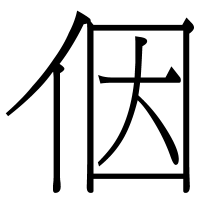
\includegraphics[height=1em]{字/⿰因}閣比漢人較早到臺灣,才會予人叫原住民。
佇歷史的文書記錄面頂,
十七世紀荷蘭佮西班牙來臺灣進前就有一个幾仔族原住民組合起來的大肚王國\cite{中研院民族所數位典藏大肚番王傳奇},
\ji{⿰因}保護\ji{⿰因}家己的土地,
抵抗荷蘭人,鄭成功政權,清國的統治,
到大甲西社事件才滅國。
到今仔日,
臺灣的原住民除了中華民國政府的原民會認定的十六族以外,
閣有誠濟猶未認定的族,
親像臺南的西拉雅佮埔里的噶哈巫……,
攏總有二三十族以上。

臺灣用的漢語主要會當分做三大種,
閩南語、客家話佮官話\cite{外省族群的母語與國語}。
閩南語佮客家話是對四百外年前開始,
佇明國、清國的福建人因為枵腹肚蹛袂落,
姑不而將駛船渡過烏水溝\footnote{又叫臺灣海峽},
來臺灣趁食。
佇清國的時陣透過政治佮經濟的力量一步一步食掉原住民的土地,
上尾佇臺灣變做上大的族群之一。

講著閩南語的文字,
定定有人問:「閩南語是欲按怎寫!?」
除了用拼音的方式寫出來以外,
閩南語有九成以上是有漢字的\cite{洪惟仁閩南語九成有漢字},
鶴佬人\footnote{閩南人。漢字有爭議,教育部無訂落來,採用洪惟仁教授的用字慣勢}祖先搬去閩越地區時,
就佮遐的壯苗族原住民通婚,
因為原住民人濟,
所以予鶴佬人同化的時留落來這一寡毋是漢語的詞,
董忠司\cite{董忠司非漢語初探}認為「查甫」佮「查某」的「查」,
「大家」佮「大官」的「大」是狀侗族的詞頭。
雖然「查」大部份人攏讀「tsa」,毋過佇臺灣漢語辭典\cite{臺灣漢語辭典}有記錄「ta」的音,佮「大」仝音。
%加注音

張光宇\cite{閩客方言史稿}研究歷史音韻學佮聲韻學\footnote{相關理論請看\ref{節:音韻學}節佮\ref{節:漢語聲韻學}節}認為,
閩南語的漢語部份是西晉後尾動亂的兩擺大移民、
唐朝陳元光𤆬兵鎮壓狀苗族原住族,
佮南宋時期文教影響,
攏總四擺移民,佮政府制度影響,
造成四層漢語語言層的閩南語。
頭前三層語言層的語音叫做白話音,
上尾第四擺後南宋音號做文讀音,
親像「石」這个字,
有「\tsoo{石}{⿳⿳⿳⿳ㄐㄧㄜ㆐ㆷ}{tsioh8}\tsoo{頭}{⿳⿳ㄊㄠˊ}{thau5}」、
「\tsoo{石}{⿳⿳⿳⿳ㄒㄧㄚ㆐ㆷ}{siah8}\tsoo{榴}{⿳⿳⿳ㄌㄧㄨˊ}{liu5}」\footnote{一種果子}、
「\tsoo{藥}{⿳⿳⿳ㄧㆦ㆐ㆶ}{iok8}\tsoo{石}{⿳⿳⿳ㄒㄧ㆐ㆶ}{sik8}」\footnote{方藥與砭石兩種藥仔}三種語音,
佇語言是規律變化的假設之下,
這个「石」字就代表上少有三層語言層。

客家話這馬佇臺灣較大腔口有「四海大平安」\footnote{四縣腔、海陸腔、大埔腔、饒平腔、詔安腔}。
鶴佬人佮客人毋管佇亞洲大陸抑是臺灣,
生活攏無遠,誠濟詞的用法攏相像,
親像閩南語講「\tsoo{頭}{⿳⿳ㄊㄠˊ}{thâu}\tsoo{前}{⿳⿳⿳ㄐㄧㄥˊ}{tsîng}」,
四縣客話講「\tsoo{頭}{}{teuˇ}\tsoo{前}{}{qienˇ}」\footnote{客話拼音會當看客話拼音\cite{客話拼音},意思會當查客話辭典\cite{客話辭典}},
閩南語講「\tsoo{好}{⿳⿳ㄏㄜˋ}{hó}\tsoo{勢}{⿳⿳ㄙㆤ˪}{sè}」,
四縣客話嘛講「\tsoo{好}{}{hoˋ}\tsoo{勢}{}{se}」。

佇臺灣的鶴佬人佮客人來臺灣佮原住民通婚,
生活中嘛濫著原住民的用詞,
親像「臺灣」是西拉雅語「Taian」或「Tayan」對外地人的稱呼\cite{台灣名稱的由來},
咱定定食著的「菝仔」嘛是平埔族話\cite{客語外來語}。

毋但原住民話,
閩南語佮客話嘛有佮別的語言交插,
像是的「六甲地」的「甲」是從荷蘭「akker」來的\cite{台甲}。
受過日本的統治,
閩南語佮客話攏有濫著日語,
親像「臭柿仔」,日語唸「\tsoo{ト}{}{to}\tsoo{マ}{}{ma}\tsoo{ト}{}{to}」,
閩南語閣會當講「\tsoo{ト}{}{*kha7}\tsoo{マ}{}{*ma1}\tsoo{ト}{}{*tooh4}」\footnote{音標有*代表外來詞,頭前兩音節kha7、ma1免閣變調},
客話講「\tsoo{ト}{}{toˇ}\tsoo{マ}{}{ma}\tsoo{ト}{}{doˋ}」,
「\tsoo{オ-}{}{oo}\tsoo{ト}{}{to}\tsoo{バイ}{}{bai}」
閩南語講「\tsoo{オ-}{}{*oo1}\tsoo{ト}{}{*too7}\tsoo{バイ}{}{*bai2}」佮「機車」,
客話講「\tsoo{オ-}{}{oˊ}\tsoo{ト}{}{do}\tsoo{バイ}{}{baiˋ}」。
會當講是臺灣的歷史攏藏佇臺灣的語言內底。

上尾一个漢語官話是中華民國政府拍輸中國人民共和國了,
⿱毛灬誠濟中國人來臺灣,
因為逐个的故鄉攏無仝\cite{外省族群的母語與國語},
民國政府就繼續用佇亞洲大陸的規範,
共北京官話的語音、白話文的用法當做基礎,
利用政府機關,教育認知\footnote{本人阿姨有佇學校講母語予人罰過錢}、…等手法佇臺灣捒,
所以華語這馬是佇臺灣是有上政治優勢的語言。
毋過這馬佇臺灣實際用的官話閣佮北京用的官話無仝款,
有加入臺灣本土的元素,是北京官話的次方言之一。
除了這三種漢語以外,
佇二次大戰了中華民國政府⿱毛灬來臺灣的人,
\ji{⿰因}的母語嘛誠濟種\cite{外省族群的母語與國語},
毋過這馬攏已經消失甲差不多矣。

為著方便起見,本論文下跤的閩南語佮客話攏是講佇臺灣用的閩南語佮客話,
官話就照中國海外華人的慣勢,稱呼佇臺灣使用的北京官話次方言做華語。
%中華民國政府就暫時叫做用政府,中華民國政府的教育部號做教育部。
本論文主要用閩南語寫,毋過會用著一寡華語佮客話。
為著格式一致,予人有法度一看就知影是啥物語言,
閩南語會用「臺羅拼音\cite{臺羅拼音}佮方言音符號\cite{華、台語注音符號溯源}」,
客話會用「客話拼音\cite{客話拼音}」,
華語會用「注音符號\cite{華、台語注音符號溯源}」。
引用的閩南語的羅馬拼音攏會轉臺羅,
毋過人名、文章名、冊名保持原樣。

\section{研究目的}
\label{節:研究目的}
%母語重要→資料無夠→需要翻譯→整理翻譯語料
最近十幾冬政府開始注重人權,講母語是人上基本的權利,
毋但國校仔國中攏開始有鄉土語言的課矣\footnote{除了本土語言以外,閣有新住民語言},
逐家嘛開始研究母語\footnote{請看\ref{章:相關研究}章},
毋過定定會拄著文字、語料、教材數量無夠的問題。

親像電視台想欲製做母語的新聞,毋過大部份攏是華語的材料;
學生想欲知影華語一句話,母語按怎講,
%文字空課
%翻譯本身
%隨身翻譯機
%數位資料無夠→翻譯重要
%外地人到臺灣,聽無臺灣話,
這時陣就會當利用華語資料攏誠濟的優勢,
共華語翻譯做母語,按呢就會解決這幾項問題。

這馬翻譯的技術已經發展到一个坎站矣,
毋過華語翻譯做母語的效果攏無蓋好,
主要是母語的語料數量無夠,
本論文就針對華語到閩南語的翻譯,
研究按怎處理數量有限的閩南語語料,予翻譯閣較好。
予後壁的人會使利用這个成果,繼續研究閩南語,
抑是會當利用這篇文章的經驗,推廣到別的臺灣語言,
上直接的,就是會當予母語使用者有閣較方便的數位環境。

%%看按怎順
%若是閣配合語音模型\footnote{請看\ref{章:語音模型}},
%都會使做一个即時口語翻譯系統。
%第一線佇學校教冊的老師需要電子化的翻譯,
%抑是關心母語的文字工作者,
%攏會使利用這个研究成果繼續做落去。

\section{語料狀況}
\label{節:語料狀況}
佇處理閩南語語料進前,都愛先了解閩南語語料的歷史。

上早的閩南語文體是明國時代流傳落來的荔鏡記戲文\cite{荔鏡記戲文研究──校勘篇},
清國時代有閣較濟的字典、歌仔冊佮教會詩歌,
日本時代開始有人感受閩南語消失的威脅,產生出臺灣話文論戰,
到中日戰爭開始,日本人禁止用漢文。%愛閣順過
中華民國政府來臺灣隨就二二八,臺灣文學因為白色恐佈,
到最近二十幾冬,閩南語才開始有大量的文章。

因為歷史誠久長,
閩南語的書寫方式有誠濟種,會當分做三種。
第一種全部用漢字,叫做全漢,
就全部用漢字表達閩南語,
因為閩南語有部份毋是漢語,
拄著這種情形逐家用的漢字攏無仝,
到最近幾冬,才有教育部以官方單位規範用字\footnote{臺灣閩南語推薦用字700字表\cite{臺灣閩南語推薦用字700字表},佇96~99年公佈修正}。

第二種是用拼音,
佇清國時期,來傳教的傳教士為著學閩南語,佮鶴佬人講話,
定一套閩南語的羅馬拼音,一般號做「教會羅馬拼音」\footnote{幾仔个版本,一般是講打馬字的版本}。
日本時期,日本政府嘛是為著統治原因,
用日本的假名來記錄\footnote{台日、日台大辭典}。
到中華民國時期,
有模仿華語注音符號的方言音符號。
最近幾十年,有主張佮英文教學系統較倚的通用拼音。
上尾教育部改教羅羅馬拼音的缺點\footnote{毋是一擺就改好,中央閣有TLPA拼音},
號做「臺灣羅馬字拼音」,後壁號做「臺羅」。
若規篇文章攏用拼音,就號做「全羅」。

面頂兩種表示法攏有缺點,
上深的漢字抑是全篇的拼音對無學過拼音的人來講較歹接受,
所以第三種就是共漢字佮拼音濫做伙,
主要是漢字,拄著較歹寫抑是揣無漢字本字的,
就寫拼音。

\section{論文貢獻}
\label{節:論文貢獻}
%第一个問題是 我們提出XX演算法
%第一个問題是翻譯語料有限,會出現「未知詞問題」,本論文提出「拄好長度斷詞」的演算法,改良斷詞的效果。
%第二个問題是翻譯語料型式真濟款,提供的資料嘛無仝,本論文提出「互相整理」的演算法,予語料格式統一。%愛號名
%第三个問題是網路語料華語閩南語濫做伙,需要共分開,以早研究攏是針對拼音字母,本論文是針對漢語方言,加特徵詞,幫助分類。
本論文主要有四个對翻譯語料的貢獻,
第一个是本論文提出「拄好長度斷詞」的演算法。
第二个貢獻是比較漢語語料樣式對翻譯的影響,
比較斷詞佮斷字翻譯模型,
佇按怎的組合之下效果上好。
第三个是提出一个自動整理漢語語料的方法,
予資訊無完整的語料庫補足資訊,
發揮上大的價值。
上尾一个是提出分類兩種漢語的方法,
免用傷濟特徵詞就會當得著袂的翻譯效果,
佇網路頂掠落來的資料就有法度分類。

\section{論文架構}
\label{節:論文架構}

%\begin{figure}
%\centerline{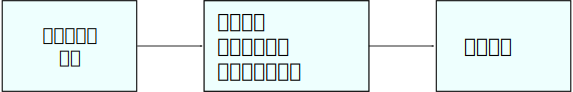
\includegraphics[keepaspectratio]{圖/規个論文}}
%\caption{本論文希望揣出自動整理語料的方法,予翻譯效果閣較好}
%\label{圖:規个論文架構}
%\end{figure}
%圖\ref{圖:規个論文架構}是這篇論文的架構,圖中央是本論文愛處理的三个問題,分別寫佇第三、四、五章。
第\ref{章:研究背景}章介紹臺灣語言的現況佮特徵,研究的動機佮論文研究的方向佮重點。
第\ref{章:相關研究}章介紹語言學研究佮技術原理。
第\ref{章:研究介紹}章定義本篇論文愛處理的問題,
第\ref{章:研究方法}章提出一寡方法,解決頂一章翻譯語料的問題。
第\ref{章:實驗結果}章做實驗而且驗證結果。
上尾的結論佮以後會當發展的方向攏記佇第\ref{章:結論佮未來發展}章。

\chapter{相關研究}
\label{章:相關研究}

\begin{figure}
\centerline{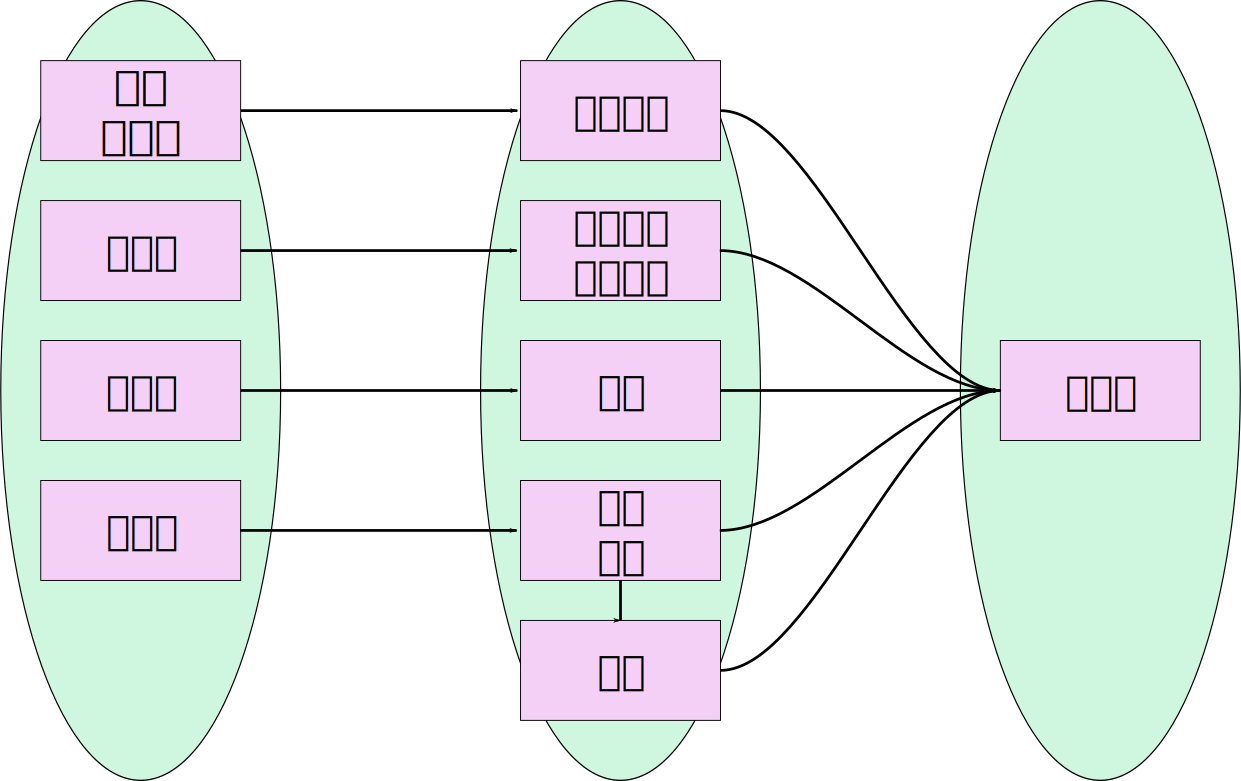
\includegraphics[keepaspectratio,width=40em]{圖/相關研究智識}}
\caption{逐門自然語言處理對應到相關的語言學}
\label{圖:相關研究智識}
\end{figure}

%漢語聲韻學→拼音系統
%語音學→語音合成、辨識
%音韻學→變調
%句法學→斷詞、剖析、翻譯
%語料庫

華語到閩南語的翻譯是自然語言處理(Natural Language Processing)\footnote{人講的話攏是自然語言}的一部份,
佇處理自然語言的時陣就需要語言相關的智識,會當簡單整理做圖\ref{圖:相關研究智識},
無仝的研究方向,愛知影的嘛無仝。
紲落來就介紹語言學佮自然語言處理的研究文獻佮母語的研究狀況。

\section{音標系統}
\label{節:音標系統}
音標系統有兩種,一種是研究語音用的記音系統,一種是予一般人拼寫用的拼音系統。

\subsection{記音系統}
\label{小節:記音系統}
研究一个語言,愛先了解伊的語音,
這時陣就需要一个標準化的記音符號。
這馬上時行的是國際語言學會(International Phonetic Association)制定的
國際音標(International Phonetic Alphabet,IPA)\cite{WIKI國際音標},
毋管記錄的語言有仝款無,只要語音的特徵仝款,就會用仝款的符號。

\subsection{拼音系統}
\label{小節:拼音系統}
記音的音標符號較濟,有的符號是較罕得看著,用起來無方便。
實際寫文章、編教材大部份會用另外的音標系統。
下跤照歷史年代簡單介紹閩南語主要三種拼音系統:

\subsubsection{臺灣閩南語羅馬字拼音}
臺灣閩南語羅馬字拼音是中華民國教育部佇2008年發佈的拼音方案,簡稱做臺羅。
伊的前身是教會羅馬字(白話字)\cite{WIKI教會羅馬字}
佮臺灣語言音標(Taiwan Language Phonetic Alphabet,TLPA)\cite{WIKI臺灣語言音標},
這馬猶原相容教會羅馬字。


\subsubsection{方音符號}
方音符號,又稱方言音符號\cite{華、台語注音符號溯源}
將華語的注音符號閣加一寡聲母、韻母佮聲調符號來標注閩南語。
是1946年朱兆祥教授設計,
佇1998年時,中華民國教育部嘛捌公告使用過。

\subsubsection{通用拼音}
余伯泉教授\ji{⿱毛灬}頭,想欲統一華語、閩南語、客語佮原住民語的拼音系統。
中華民國教育部佇2002年到2008年規定華語通用拼音當做譯音標準。

\subsubsection{音標比較表}
國際音標 臺羅 方音 通用 例字


\section{語音學}
\label{節:語音學}

\begin{table}
\caption{元音表}
\label{表:元音表}
\centering
\begin{tabular}{c|ccc}
\diaghead{\theadfont Diag ColumnmnHead II}{喙舌懸低}{喙舌前後}
%喙唇扁/圓 
& 頭前 & 中央 & 後壁\\
\hline
懸 & [i] & [ɨ] & [u]\\
中懸 & [e] &  & [o]\\
中 &  & [ə] & \\
中低 & [ɛ] &  & [ɔ]\\
低 & [a] &  & [ɑ]\\
\end{tabular}
\end{table}

\begin{table}
\caption{輔音表}
\label{表:輔音表}
\centering
\begin{tabular}{c|ccc}
\diaghead{\theadfont Diag ColumnmnHead II}{發音方式}{喙舌所在}
& 喙唇 & 中央 & 後壁\\
\hline
清塞音 & [i] & [ɨ] & [u]\\
濁塞音 & i & ɨ & u\\
鼻音 & [e] &  & [o]\\
邊音 &  & ə & \\
擦音 & ɛ &  & ɔ\\
\end{tabular}
\end{table}

\begin{table}
\caption{音節分析}
\label{表:音節分析}
\centering
\begin{tabular}{cccccc}
字 & 聲母 & \multicolumn{3}{c}{韻母} & 聲調\\
 & & 介音 & 主要元音 & 韻尾 &\\
\tsoo{良}{⿳⿳⿳ㄌㄧㆲˊ}{liong5} & [l] & [j] & [o] & [ŋ] & 5\\
\tsoo{媠}{⿳⿳⿳ㄙㄨㄧˋ}{sui2} & [s] & [u] & [i] & & 2\\
\tsoo{遠}{⿳⿳ㄏㆭ˫}{hng7} & [h] & & [ŋ̩] & & 7\\
\tsoo{意}{⿳ㄧ˪}{i3} & & & [i] & & 3\\
\end{tabular}
\end{table}

語音學(Phonetics)主要討論喙舌的運動方式佮語音的物理性質。

前國際語言學會會長John Ohala捌講過:
「語音變化是連續的(Continuous),為著研究只好假設做離散特徵(Discrete)的音素(Phoneme)。」
可比講「\tsoo{狗}{⿳⿳ㄍㄠˋ}{kau2}」,
音標寫做[kau],
實際上[k]佮[a]、[a]佮[u]中央有誠濟過渡的音,
毋過過渡的音實在傷濟,
無法度一个一个寫出來,
只好用[k]、[a]佮[u]三个符號代表「\tsoo{狗}{⿳⿳ㄍㄠˋ}{kau2}」的音標。

語音會當用氣流有順無,
大略仔分做元音(Vowel)佮輔音(Consonant)。
表\ref{表:元音表}是幾仔个閩南語定用的元音,
會當看著[i]佮[u]攏是喙舌較懸發的音,
而且喙舌佇i發音時比u發音閣較頭前,
這嘛影響著\ji{⿰因}的頻譜(Frequency Spectrum),
[i]佮[u]共振鋒(Formant)嘛小可無仝。
[i]佮[u]喙型嘛無仝,
唸「\tsoo{ㄨ}{}{u}」的時陣喙尖尖,
唸「\tsoo{ー}{}{i}」的時陣喙較平,
嘛影響著語音的變化。
%裂 sai sai:伊笑甲~~~
%裂喙:伊笑的時陣攏會~~

佇分析漢語的時,
會親像表\ref{表:音節分析}仝款,
共音節拆做聲母、韻母佮聲調來看,
韻母閣會當分做介音、主要元音佮韻尾。
毋過愛注意,
這个分析只是方便研究,
聲母、韻母的元素佮聲調猶原會互相影響。


若了解語音學,
就會當知影語音變化的道理,
支持音韻學的理論。

\section{音韻學}
\label{節:音韻學}

\begin{table}
\caption{閩南語上細配對}
\label{表:上細配對}
\centering
\begin{tabular}{c|cc}
& 喙唇 & 中央\\
\hline
元音、鼻化音 & [i](\tsoo{異}{⿳ㄧ˫}{i7}) & [ĩ](\tsoo{院}{⿳ㆪ˫}{inn7})\\
配合濁聲母 & [bi](\tsoo{味}{⿳⿳ㆠㄧ˫}{bi7}) & [mĩ](\tsoo{麵}{⿳⿳ㄇㄧ˫}{mi7})\\
\end{tabular}
\end{table}

現代的音韻學(Phonology)是對Ferdinand de Saussure\cite{de2011course}提出語言學研究,
必須分做共時(Synchronic Phonology)佮歷史(Diachronic Phonology)兩種音韻學。

\subsection{共時音韻學}
\label{小節:共時音韻學}
共時音韻學就是對一个時間的一个語言,
%討論變化,心中所想音檔→唸出來。
討論「頭殼底所想的音」到「唸出來的聲音」的語音變化。
佇討論語音進前,
咱就愛先訂出共時的語音單位,
定用的語音單位是音素。
音素代表一个人「頭殼底」,
對一个語言的「語音單位」。
愛判斷兩个音是毋是仝一个音素,
會當來揣「上細配對」。
可比講表\ref{表:上細配對}第一逝,
一般元音佮鼻化元音會當分出無仝的字,
所以[i]佮[ĩ]對人來講是辨識語音的單位,
是無仝的兩个音素。

\begin{equation}
\label{式:閩南語濁聲母變化式}
B\rightarrow\left\{\begin{matrix}
[b], & 佇一般元音頭前\\ 
[m], & 佇一般鼻化音頭前
\end{matrix}\right.
\end{equation}
\begin{table}
\centering
\caption{閩南語濁聲母無鼻化的選擇}
\label{表:閩南語濁聲母無鼻化的選擇}
\begin{tabular}{c|cc|c}
Bi+無鼻化 & 元音符合鼻音要求 & 規个音節鼻化一致 & 上好的選擇 \\
\hline
{[}bi{]} & & & ←是\tablefootnote{佇優選理論內底,←代表上好的選擇}\\
{[}bĩ{]} & *!毋是\tablefootnote{佇優選理論內底,*代表違反限制,!代表出局} & *毋是\cellcolor{gray}\tablefootnote{佇優選理論內底,殕色底代表選擇出局,毋免比} & \\
{[}mi{]} & & *!毋是 & \\
{[}mĩ{]} & *!毋是 & \cellcolor{gray} & \\
\end{tabular}
\caption{閩南語濁聲母有鼻化的選擇}
\label{表:閩南語濁聲母有鼻化的選擇}
\begin{tabular}{c|cc|c}
Bi+有鼻化 & 元音符合鼻音要求 & 規个音節鼻化一致 & 上好的選擇 \\
\hline
{[}bi{]} & *毋是 & \cellcolor{gray} & \\
{[}bĩ{]} & & *毋是 & \\
{[}mi{]} & *毋是 & *毋是\cellcolor{gray} & \\
{[}mĩ{]} & & & ←是\\
\end{tabular}
\end{table}

毋過看第二逝,
濁輔音佇[i]頭前是塞音[b],
佇[ĩ]頭前是變化鼻音[m],
因為無對比通證明[b]佮[m]有分辨字的能力,
所以[b]佮[m]對人來講「可能」是仝一个語音單位,
會當歸類做一个音素$B$\footnote{這个符號用m、b攏會使,伊只是代表一个音素},
只是$B$佇無仝的所在會唸無仝的音。

音韻學家就想欲揣出「頭殼底所想的音」到「唸出來的聲音」的關係,
討論為啥物面頂的$B$有時唸[b],有時陣唸[m],
目前較大的有衍生音韻學(Generative Phonology)佮優選理論(Optimality Theory)兩大派。

\subsubsection{衍生音韻學}
衍生音韻學是希望揣出的對應音韻規則(Phonological Rule),
親像面頂[b]佮[m]的問題會當看閩南語濁聲母變化規則\ref{式:閩南語濁聲母變化式},
$B$若後壁是一般元音,就變做[b],
若後壁是鼻化音,就變做[m]。

\subsubsection{優選理論}
第二派優選理論是揣出一寡人類語言通用的現象,
而且共這現象,
照重要程度排先後,
去揀人為啥物愛唸這个音。

可比講[b]佮[m]的問題,
咱有「元音符合鼻音要求」佮「規个音節鼻化一致」\cite{yip1996lexicon}兩个現象,
第一个現象「元音符合鼻音要求」是希望主要元音愛符合頭殼內有鼻音無鼻音的條件,
第二个現象「規个音節鼻化一致」是希望音節全部的音素,
\ji{⿰因}鼻化狀況是仝款的,
而且第一个現象比第二个現象優先,
若第一个現象無過,就免比第二个現象。

親像表\ref{表:閩南語濁聲母無鼻化的選擇},
假設頭殼底想的是「Bi+無鼻化」,
咱先產生[bi]、[bĩ]、[mi]、[mĩ]四个選擇\footnote{選擇其實閣有pi、pĩ、…無限濟个,\ji{⿰因}會用別的現象揀掉。為著簡單說明就無寫出來。},
其中[bĩ]佮[mĩ]違反第一个現象,
[bĩ]佮[mĩ]予人揀掉,
[bĩ]、[mi]違反第二个現象,
毋過因為[bĩ]早就違反第一个現象,
無需要閣判斷第二个現象,
所以第二个現象揀掉[mi]
上尾賰[bi],就是上好的選擇。
表\ref{表:閩南語濁聲母有鼻化的選擇}是「Bi+有鼻化」的例,
伊佇第一个現象揀掉[bi]、[mi],
第二个現象揀掉[bĩ],
上尾賰[mĩ]是上好的選擇。

\subsection{歷史音韻學}
\label{小節:歷史音韻學}
\begin{table}
\caption{閩南語低元音提昇過程\cite{hsieh2012low}}
\label{表:閩南語低元音提昇過程}
\centering
\begin{tabular}{ccc}
階段  & 音值 & 來源 \\
Stage 1 & jan/jat\tablefootnote{[i]的介音寫做[j]} &  Doty (1853), dictionary of Amoy dialect\\
Stage 2 & jan/jat &  Luo \& Zhou’s fieldwork in 1930 (L\&Z 1975)\\
Stage 3 & jen/jet & Taiwanese and some Southern Min dialects\\
Stage 4 & en/et & New forms among young Taiwanese speakers\\
\end{tabular}
\end{table}
\begin{equation}
\label{式:閩南語咸攝三等變化式}
[jaC]\rightarrow[jeC]\rightarrow[eC],若C\in\left\lbrace n,t\right\rbrace 
\end{equation}
\begin{equation}
\label{式:閩南語非咸攝三等變化式}
[jaC]\nrightarrow[jeC],若C\not\in\left\lbrace n,t\right\rbrace
\end{equation}
%[ja]\nrightarrow[je]

歷史音韻學是討論語言長期的變化佮語言互相的影響,
這个變化無一定是講話的人講無清楚,
嘛有可能是因為音相倚,
聽話的人聽毋著,
一緣一緣的人沓沓仔改變的。

親像表\ref{表:閩南語低元音提昇過程}記錄
閩南語「\tsoo{先}{⿳⿳ㄒㄧㄢ}{sian1}」佮「\tsoo{節}{⿳⿳⿳ㄐㄧㄚㆵ}{tsiat4}」韻母
這兩百冬的變化,
所以咱會當共這變化整理做規則\ref{式:閩南語咸攝三等變化式}。
除了寫出規則以外,
閣愛需要用語音學解釋為啥物會按呢生,
是因為頭前有介音[j],
喙舌佇較懸較頭前的所在\footnote{元音的所在會當看表\ref{表:元音表}},
後壁[n]佮[t]是舌尖音,
喙舌嘛是佇較懸較頭前的所在\footnote{舌尖音佮[i]、[j]的位較倚,讀者會當唸看覓[in]、[en]佮[an],觀察喙舌的變化},
予原本喙舌較低的[a],
變做喙舌較懸較頭前一寡的[e]。

毋過觀察別的韻煞無這種變化,
親像規則\ref{式:閩南語非咸攝三等變化式},
「\tsoo{閃}{⿳⿳⿳ㄒㄧㆰˋ}{siam2}」、「\tsoo{雙}{⿳⿳ㄒㄧㄤ}{siang1}」猶原是[jam]佮[jaŋ]。
用語音學的角度來看,
干焦頭前介音[j],無後壁的韻尾配合,
無法度予[a]變懸變做[e]。


\section{漢語聲韻學}
\label{節:漢語聲韻學}
聲韻學是研究漢語自古到現代,方言的變化佮語音規律,
算是專門研究漢語的歷史語言學。

自三國南北朝時就有韻冊\footnote{李登《聲類》、呂靜《韻集》},
韻冊會記錄逐个字的反切,共仝韻母的字下做伙。
反切是古代中國用的記音方式,反切記音需要記兩个字,
一字代表聲母,一字代表韻母,
親像閩南語的「\tsoo{東}{⿳ㄉㄤ}{tang}」會用「\tsoo{端}{⿳ㄉ}{t}」「\tsoo{通}{⿳ㄤ}{ang}」表示。%用「車」?

到這馬上早上完整的文獻是宋國官修的廣韻\cite{2002廣韻注漳州漢音}\cite{2010新校互註宋本廣韻},
伊是綜合中國北方佮南方的語音系統。
嘛因為廣韻是綜合各地的系統,
伊記錄的反切嘛會當佇無仝的漢語方言用,
除了閩南語的「東」會當切做「端通」
華語的「\tsoo{東}{⿳⿳ㄉㄨㄥ}{}」嘛會當反切做「\tsoo{端}{⿳ㄉ}{}」「\tsoo{通}{⿳ㄨㄥ}{}」

嘛因為韻冊記錄是反切,毋是實際發音音值,
誠濟聲韻學家音韻學的理論,佮現代方言的材料,
來推測古早漢語的實際發音,
擬一套發音系統。

%狗頭後
%師詩斯


\section{句法學}
\label{節:句法學}
討論啥物是詞、詞的用法。句型

陸XX

\section{變調}
\label{節:變調}

準做想欲共臺語的字變做臺語的聲音,咱必須佮字,先標一對一斷詞,揣出音標。
但是臺語的變調是足複雜的,無法度予HTS內底的決策樹來做
所以愛先用另外一支程式專門來變調
楊允言教授就有做過\cite{iunn:台語變調系統實作研究},伊是用規則來確定變調的狀況,毋過伊用的語料無蓋濟,若數量一濟,規則式的變調會較歹處理。
變調嘛會當用機器學習的方法來做,共規則式用掉的特徵做伙下入去,看佗一个分類模型會較好,毋過伊上大的好處就是伊管理方便,免拄著啥物新語料,規則就愛全部重改,伊干焦需要共新語料加入重訓練就好矣,毋過伊的內部試驗就無保證一定著矣。

\section{語音辨識}
\label{節:語音辨識}
語音辨識就是共聲音轉做文字,會當用佇語音指令佮問答系統\footnote{親像蘋果公司的Siri}。
主流的做法是先共聲音轉做MFCC特徵
%\footnote{用MFCC特徵\cite{MFCC特徵}是因為實驗的效果上好\cite{MFCC上好}}
,
閣配合音檔的文本,
用隱性馬可夫模型\footnote{語音的變化當作狀態的轉移,而且聲音訊號是連續,無固定長度的特性。請看\ref{小節:隱性馬可夫模型}節。}
佮一个分類器\footnote{請看\ref{節:分類器}節}
訓練出辨識模型。

這方面的開源工具有HTK佮Kaldi:

\subsection{HTK}
\label{小節:HTK}
HTK全名號做Hidden Markov Model Toolkit\cite{HTK網頁},
發展的時間較早\footnote{對1989年到最近上新的2009年版本},
伊主要用\ref{小節:高斯混合模型}的高斯混合模型當做分類器。

HTK的模型訓練腳本\footnote{會當參考附錄\ref{章:臺灣言語工具}的臺灣言語工具,內底有提共HTK訓練佮使用的腳本},
一開始會先照文本的音,共音檔平均切做一个一个,
HTK流程圖~~

%決策樹
%wfst

\subsection{Kaldi}
\label{小節:Kaldi}
Kaldi\cite{Kaldi:Povey_ASRU2011}是較新的工具,
除了訓練一開始嘛是佮HTK仝款用高斯混合模型以外,
伊訓練後壁閣加入其他演算法,
效果比HTK閣較好。
%伊上大的特色是後壁分類器閣用深層類神經網路\cite{DNN},

%SGMM

\section{語音合成}
\label{節:語音合成}
語音合成是佮文字轉做聲音,佮語音辨識顛倒反,
親像車站廣播,有聲冊攏是語音合成的應用。
這馬時行的做法有兩種:

\subsection{模型合成}
\label{小節:模型合成}
這个方法頭一步是
先用人工抑是語音辨識軟體標記音檔的音,
共全部的音的特徵訓練出一个模型,
等欲合聲音時,才閣照模型的特徵,
用合成器合聲音出來。


\subsubsection{HTS}
\label{小節:HTS}
這方面開源軟體有HTS(HMM-based Speech Synthesis System)\cite{HTS網頁},
伊是對HTK修改來的。
用mgc、lf0、duration做聲音特徵,

伊訓練方式,
伊一个聲音會分做5个state\footnote{下跤講著的5狀態、三連音,攏是參數,毋是固定的},
逐个state有一个高斯模型,
伊會先訓練逐个音的初步模型,
閣來訓練三連音模型,
閣用決策樹共相倚的音綁做伙。

合的時陣才閣查決策樹,
共mgc、lf0、duration查出來,
閣用合成器合語音出來。

HTS只需要3000~7000句的訓練語料,
伊的輸出語音,
韻律攏袂\ji{⿰禾黑},
毋過因為聲音先轉做特徵,
特徵閣轉轉語音,
聲音的品質比原本的聲音會較\ji{⿰禾黑}一寡。

%伊需要音檔,標記發音內容的音檔,閣有音類的問題集。設計標仔。
%標仔的時間會使對HTK訓練。
%根據經驗,3000句會使,5000句普通,7000句上好。

\subsection{接聲音合成}
\label{小節:接聲音合成}

優點是聲音品質誠好,缺點是語料愛有夠濟,因為

\subsection{語音合成相關系統}
\label{小節:語音合成相關系統}
佇1999年林川傑就提出閩南語翻譯佮語音合成系統\cite{中文到閩南語之線上翻譯及閩南語之語音合成},

\section{斷詞}
\label{節:斷詞}
有一寡語言現象是佮詞有關係,
親像閩南語的變調,
毋過漢語語句的文本,
定定是一定一字無分開,
就看袂出來倒底佗一字佮佗一字是一个詞,
所以就需要斷詞,
共詞佮詞分開,
後壁的應用才有法度繼續落去。



華語這方面有中研院中文斷詞系統(CKIP)\cite{CKIP論文}。

閩南語斷詞的標準,
自誠早以前就有人討論矣\cite{台語斷詞原則討論},
教育部嘛有出「臺灣閩南語羅馬字拼音方案連字符使用原則」\cite{臺羅拼音},
定義連字符的標準。

%斷詞的標準有誠濟種,為著方便,以教育部的「臺灣閩南語羅馬字拼音方案連字符使用原則」的連字符當做一个詞,若「tsiah8 png7」(食白米飯的意思),當做兩个詞,「tsiah8-png7」(食物件的意思),當做一个詞。


%斷詞方法:長詞優先、配合語言模型、統計式、馬可夫、詞性

\subsection{長詞優先斷詞}
\label{節:長詞優先斷詞}

%定看著的斷詞方法有上長詞優先\footnote{(FMM)},伊的做法是自頭開始,看頭前幾个字是毋是會當揣著一个佇辭典的詞,若會使,就揀上長的彼个,…
%解釋比如說,『我想要吃飯』可以切成『我,想,要,吃,飯』『我,想要,吃飯』『我,想要吃飯』『我想要,吃飯』『我想要吃飯』,其中,能夠在字典找到詞的切割方式有『我,想,要,吃,飯』『我,想要,吃飯』,

\section{詞性標記}
\label{節:詞性標記}
\cite{iunn:利用統計方法及中文訓練資料處理台語文詞性標記}

\section{剖析}
\label{節:剖析}
斷詞了後毋知詞佮詞的關係
所以剖析
會當用佇翻譯佮語意分析(用佇問答系統)
楊允言教授有做過\cite{台語文語法結構樹建置}。
\section{翻譯}
\label{節:翻譯}
這馬電腦時行的翻譯方式是統計式機器翻譯(statistical machine translation),
這是對1993年Brown用數學證明\cite{brown1993mathematics}開始,
一直發展到這馬。
統計式機器翻譯會當分做對齊模型(alignment model)、語言模型(language model)佮解碼器(decoder)三个部份:

\subsection{對齊模型}
\label{小節:對齊模型}
對齊模型的功能是予解碼器知影詞愛按怎翻譯,
可比講是一个雙語的辭典。

對齊模型有分斷詞對齊佮剖析樹對齊兩種,下跤用斷詞對齊說明伊的原理。

先準備一組一組的華語閩南語平行語料,
親像「我 要 吃飯」和「我 欲 食 飯」,
紲落來產生語詞對照表。
華語詞的「要」,會對應到「我」、「欲」、「食」、「飯」閩南語詞,
經過大量的平行語料,
上尾知影華語的「要」定定對應著閩南語的「欲」,
也就是共對應頻率懸的組合留落來。
%改例

開源工具GIZA++\cite{och2003systematic}實作Brown 1993的演算法,
而且這馬嘛有支援多核心的MGIZA\cite{gao2008parallel}。

\subsection{語言模型}
\label{小節:語言模型}
第二部份是語言模型(language model),伊是欲用來判斷一句話是好是\ji{⿰禾黑}。

%加數學解釋
伊的做法是去記錄逐个詞後壁定定會接啥物詞,
若有一句話是「…欲 食…」,有「欲」佮「食」兩个詞,
咱知影「…欲 食」的後壁接「飯」比「…欲 食」的後壁接「湯」的機率較大,
也就是講「欲 食 飯」連紲詞比「欲 食 湯」連紲詞機率大,
若語言模型一擺看「欲 食 飯」三个詞,
就是三連紲詞模型(3-grams model)。
語言模型判斷一句話,伊出現的機率有偌大,就是看這句話伊內底連紲詞的機率是偌大。
%改例

這方面的工具有IRSTLM\cite{federico2008irstlm}、
SRILM\cite{stolcke2002srilm}佮
KenLM\cite{Heafield-estimate},
其中IRSTLM佮KenLM是LGPL開放授權,
SRILM是學術授權。

\subsection{解碼器}
\label{小節:解碼器}
上尾一部份是解碼器,
提面頂講的對齊模型、語言模型,
來翻譯華語到閩南語。

因為翻譯的問題毋是多項式時間(NP problem)會當解出來的,
所以解碼器袂使硬算全部的可能,
必須用有效率的演算法來翻譯。

上有名的開源程式就是Moses\cite{Koehn:2007:MOS:1557769.1557821},
伊整合對齊模型佮語言模型的介面,
閣有專工的訓練包通使用\cite{Moses訓練包}。

\subsection{評分方式}
\label{小節:評分方式}

翻譯大部份攏用BLEU(Bilingual Evaluation Understudy)來評分,
伊用連紲詞的概念來評分,
$BLEU=100\times{e^{\max{0,\frac{\textit{結果-答案長度}}{\textit{結果長度}}}}}\times{\sum_{n=1}^{4}(\textrm{n連紲詞})^{\frac{1}{4}}}$\cite{BLEU程式}。
%改cite

準若翻譯的答案是「這 幾 工 寒流 閣再 展威」,咱有兩个翻譯的結果,翻譯結果一「這 幾 工 寒流 有 展威」佮結果二「寒流 這 幾 工 閣再 展威」,請看表\ref{表:範例BLEU分數},答案有「這 幾 工」、「幾 工 寒流」、「工 寒流 閣再」佮「寒流 閣再 展威」4个三連紲詞,結果一有出現2个,所以結果一的三連紲詞分數是2/4,結果二有出現1个,分數是1/4。因為結果二無對應的四連紲詞,伊的分數都比結果一低。

\begin{table}
\caption{翻譯結果一「這 幾 工 寒流 有 展威」佮翻譯結果二「寒流 這 幾 工 閣再 展威」對答案「這 幾 工 寒流 閣再 展威」的分數}%
\label{表:範例BLEU分數}
\centering
\begin{tabular}{|c|cccc|c|}
\hline
翻著的數量 & 一連紲詞 & 兩連紲詞 & 三連紲詞 & 四連紲詞 & BLEU分數\\
\hline
結果一 & 5/6 & 3/5 & 2/4 & 1/3 & 53.73\\
\hline
結果二 & 6/6 & 3/5 & 1/4 & 0/4 & 0.00\\
\hline
\end{tabular}
\end{table}


\section{語料庫}
\label{節:語料庫}
自然語言處理需要語料才有法度訓練模型,
就需要語料庫共語料存起來。

\begin{table}
\caption{自然語言處理技術需要的語料庫}
\label{表:自然語言處理技術需要的語料庫}
\centering
\begin{tabular}{lc}
技術 & 語料樣式 \\
變調 & 原始文本、本調音標佮變調音標 \\
語音辨識 & 濟人音檔佮對應文本 \\
語音合成 & 孤人音檔佮對應文本 \\
斷詞 & 斷詞的語料 \\
剖析 & 剖析樹 \\
翻譯 & 兩種語言的平行語料 \\
\end{tabular}
\end{table}

有的語料庫是純文字的資料庫,
嘛有存音檔的語料庫,
愛看需求,定看著的技術會當參考表\ref{表:自然語言處理技術需要的語料庫}。

\subsection{閩南語語料種類}
\label{節:閩南語語料種類}

\begin{table}
\caption{閩南語語料種類比較表}
\label{表:閩南語語料種類比較表}
\centering
\begin{tabular}{lcc}
種類 & 範例 & 備註\\
全漢 & 我欲食飯 & 全部漢字\\
全羅 & gua2 beh4 tsiah8-png7 & 全部羅馬拼音,有斷詞資訊\\
漢羅 &我beh4食飯 & 漢字拼音濫咧用\\
\end{tabular}
\end{table}

閩南語是漢語的一支方言,
大部份的字攏會當揣著漢字,
毋過閩南語嘛毋是純漢語,
有的字無對應的漢字。

有的人慣勢全部用羅馬拼音創作,
這種寫法號做「全羅」。
嘛有人慣勢全部用漢字創作,
號做「全漢」
毋過有的字無法度揣著對應的漢字,
全漢實際上的拄著造字、揣字的困難,
為著創作方便,
知影的字用漢字寫,
賰的用音標寫落來,
號做「漢羅」。
詳細會當看表\ref{表:閩南語語料種類比較表}的範例。

\subsection{閩南語語料-新聞語料庫}
\label{節:新聞語料庫}
華語閩南語雙語語料庫\footnote{\url{http://icorpus.iis.sinica.edu.tw/}}(後壁用「新聞語料庫」稱呼)是何澤政\footnote{一九七零年代出世,臺中烏日人}對民國九十七年十一月初六開始,逐工揣兩篇華語新聞,先斷句,後尾翻譯做閩南語教會全羅。親像原本的新聞「這幾天寒流再度發威」,翻譯做「tsit4-kui2-kang han5-liu5 koh-tsai3 tian2-ui」(這幾工寒流閣再展威)\footnote{原文是教會羅馬字,為著文章一致,以教育部的臺羅書寫}。
新聞語料庫的翻譯罕得改變用詞的先後,親像面頂的「這幾天寒流再度發威」,較袂翻做「寒流這幾工閣再展威」,除非照華語用詞先後翻譯的結果無順,才會調整。

澤政佇語料內底用
「挕捒 hinn3-sak4」\footnote{挕捒意思共物件擲掉、放捒,嘛就是華話的「丟棄」,例句甲(家己做的):這支筆好好,為啥物愛共伊挕捒。例句乙(Tek-hôa,Nah ē teh批判民進黨?,\url{http://taioan-chouhap.myweb.hinet.net/089.htm}):民進黨接續李登輝的路線, 繼續加強黨國時代權力者, 倚附者佮既得利益者的優勢,毋是共刜挕捒。}
、
「作孽」\footnote{
青-少-年|tshing1-siau3-lian5 作-孽|tsok4-giat8 跤-踏-車|kha1-tah8-tshia1 擲|tan3 落|loh8 河-中|ho5-tiong1。

愛耍手賤,華語的「惡作劇」。例句甲:叫你莫摸你閣摸,誠實手賤愛作孽!(家己做的)例句乙:你這个作孽囡仔,你是按怎沐甲一身軀烏趖趖?(惠光,天真瀾漫,\url{http://ip194097.ntcu.edu.tw/nmtl/DADWT/thak.asp?id=992})}
本土的詞以外,伊嘛會配合這馬發生的代誌,用較時行的閩南語,親像
「喙罨」\footnote{華語的「口罩」}、
「心肌梗窒」\footnote{心|sim1 肌|ki1 梗|king2 窒|that4,華語的「心肌梗塞」}、
「自來水」\footnote{閩南語較古典的用法,會號做「水道水」}、…。
而且除了現代閩南語,澤政伊閣會去查台華線頂辭典\footnote{\url{http://ip194097.ntcu.edu.tw/iug/Ungian/SoannTeng/chil/Taihoa.asp}}
選擇較古典的用詞\footnote{台華線頂辭典是古早語料,一个詞若台華線頂辭典查有,教育部辭典查無,就當做伊是較古典的詞},親像
「𤺪|sian7 篤-篤|tauh4-tauh4」\footnote{熱-天|juah8-thinn1 高-溫|ko1-un1 炎-熱|iam7-juah8 規-工|kui1-kang1 𤺪|sian7 篤-篤|tauh4-tauh4 。|。}、「鬥-贊-手|tau3-tsan3-tshiu2」\footnote{佇|ti7 三|sam1 一-一|it4-it4 大-地-動|tua7-te7-tang7 慷-慨|khong2-khai3 鬥-贊-手|tau3-tsan3-tshiu2 ,|,}。

拄著外來詞,澤政嘛會選擇保留原文,拄著華語的「歐巴馬」佮「西藏」,會翻轉去英文「Obama」、「Tibet」。

斷詞組

加漢字,

若源頭是日本話外來詞,就會直接用教羅寫出來,請看

\subsection{閩南語語料-教育部辭典}
\label{節:教育部辭典}
這章按算加入教育部辭典佮數位典藏兩个語料庫,教育部辭典全名「臺灣閩南語常用詞辭典」\footnote{\url{http://twblg.dict.edu.tw/holodict_new/}},正式版是100年上線,伊有25892的詞條\footnote{1021230申請到的版本},內底誠濟生活的用語,大部份詞條攏有漢字、音標、解釋、佮例句。的翻譯。
嘛因為伊有漢字佮音標,就會當共遮的漢字佮音標收集起來,當做用字參考的字典,
這个辭典是教育部編的,當然漢字有照教育部家己的規範\footnote{臺灣閩南語推薦用字700字表,佇96~99年公佈修正}來寫,所以伊內部的用字前後有一致,為著翻譯的效果佮使用者的方便,就共教育部辭典的用字當做標準,若有用字佮教育部的用字無仝的,就改做教育部的用字。//閣愛順過

伊的例句,除了閩南語漢字佮音標以外,閣有敆華語的翻譯,親像表\ref{表:教育部辭典例句},漢字佮音標的對應會使提去做用字參考的字典,音標的部份會當提來斷詞,訓練語言模型,閩南語佮華語的對應會使提來做平行語料。這例句的語料是非常完整,攏總有8XXX句。
\begin{table}
\caption{教育部辭典例句}
\label{表:教育部辭典例句}
\centering
\begin{tabular}{l}
彼个查某囡仔真媠。 \\
Hit ê tsa-bóo gín-á tsin suí.\\
那個女孩子很漂亮。\\
\end{tabular}
\end{table}

除了一般的詞條以外,教育部辭典嘛有收一寡俗語、臆謎猜,攏做388句做附錄句。
因為附錄句干焦提供解釋,所以無法度提來做平行語料,毋過會使提來訓練語言模型。

台語文數位典藏資料庫\footnote{\url{http://xdcm.nmtl.gov.tw/dadwt/pbk.asp}}(下跤號做數位典藏)是國家臺灣文學館收集1885~2006年的語料,攏總2167篇。
照時代分做清國時期170篇、日治時代490篇,民國統治1507篇。內底嘛有照語料形式分做四類,有詩387條、散文1127篇、小說387篇、劇本49篇。攏總416343句。

因為伊是百外冬的語料庫,較古早的語料,用詞就較古典, %//閣再加

\subsection{閩南語語料-數位典藏}
\label{節:數位典藏}
數位典藏的來源語料百百款,臺文館⿰因為著格式統一,就替原底是全漢抑是漢羅的語料補全羅拼音\footnote{有時陣劇本邊仔的解釋會用漢字,親像「(福哥仔出場)」},若原本是全羅,就請人拍漢羅,會當看表\ref{表:數位典藏語料},拍漢羅的時,⿰因若知影漢字,就會拍漢字,賰的外來語,抑是較本土的語詞就會用音標來拍。
伊有的語料是一句對齊一句,有的是一段對齊一段。

\begin{table}
\caption{數位典藏語料漢羅、全羅對照}
\label{表:數位典藏語料}
\centering
\begin{tabular}{l}
漢羅:Koh m7知u7危險.........., \\
全羅:Koh m7-tsai u7 gui5-hiam2..............., \footnote{數位典藏內底原本是白話字(教會羅馬拼會),為著讀者方便,攏改做教育部的臺羅}\\
\end{tabular}
\end{table}


\subsection{閩南語語料-TGB通訊臺灣組合}
\label{節:TGB通訊-臺灣組合}
TGB通訊\footnote{\url{http://taioan-chouhap.myweb.hinet.net/}}是學生台灣語文促進會對1999年10月開始\footnote{\url{http://taioanchouhap.pixnet.net/blog/post/32374696}}一個月一期的刊物。頭前60期以閩南語為主,61期有提供華語對照,有時陣閩南語句內底會濫一寡華語詞,形式較無固定

因為有閩南語、有華語佮臺華平行語料,嘛閣有濫做伙的, 誠濟種實際會拄著的情形會當提來做判斷語言的語料。
有的時陣閩南語佮華語濫做伙,先定義啥物情形算閩南語,啥物情形算華語

用人工分

主要語句是閩南語,有一兩个詞是華語嘛是算閩南語
閩南語

聽人講 khah 早有出現過『小蜜蜂』
我 beh tńg 來種作 ! ── 記 0312 Truku 反亞泥 ‧ 還我土地運動
有台灣味 ê 繪本──《我和我的腳踏車》 .

華語
華語閩南語攏通的算華語
有華語完整的一句話就算華語
毋是華語嘛毋是閩南語,親像英文、日語、…

「 糟了 ,是工地火燒厝, 緊轉去打 火 ! 」建設公司 的 工地主任 從手機接到消息,通話結束後就帶著那群混混先離開了。
『聽說妳最近遇到什麼問題 , 是不是 ? 怎麼了 ? 』好性地 ê QA 繼續問--落-去 .
去越南胡志明市 4 工/越南胡志明市四日行 @Gio̍k-hōng

\subsection{閩南語語料腔口統計佮處理}
\label{小節:閩南語語料腔口統計佮處理}

\section{語料收集整理}
\label{節:語料收集整理}
佇這个網路的時代,收集語料上緊的方法就是去網路面頂掠。看圖XX,先共閩南語專門的字詞擲去搜尋引擊\footnote{親像Google、Bing},閣照揣著的網頁去掠相關的閩南語。
閩南語的網頁內底除了閩南語以外,有可能閣濫一部份的華語,為著莫予華語語料影響著閩南語模型,所以愛想辦法共臺華兩種語言分開。分開了後

%圖:關鍵詞 引擊 網址 掠網頁 網頁html 轉文字 一句一句的語料 判斷語言 閩南語/華語 對齊

\begin{figure}
\centerline{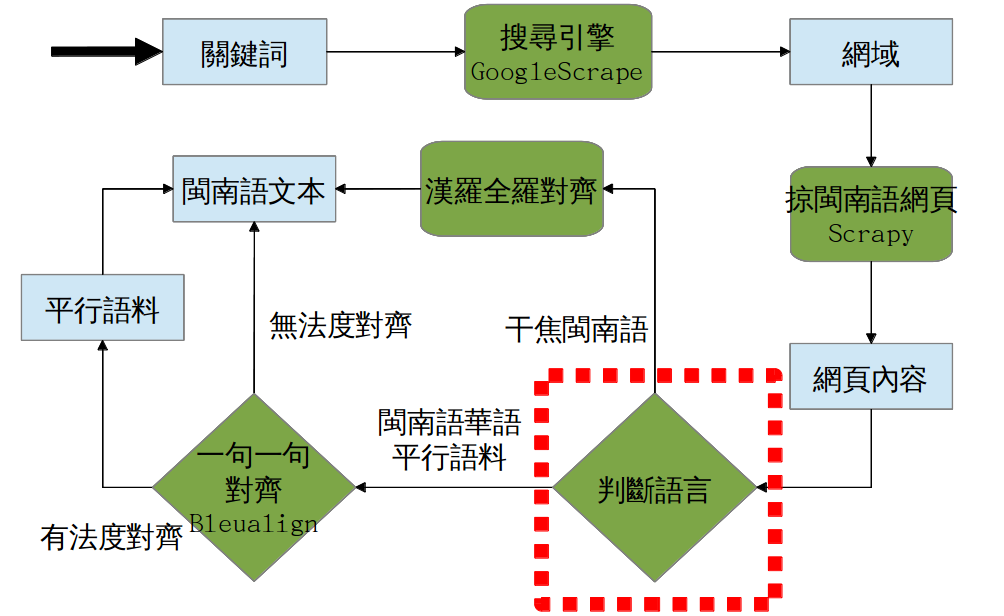
\includegraphics[keepaspectratio,width=40em]{圖/網路語料庫結構}}
\caption{網路語料庫}
\label{圖:網路語料庫結構}
\end{figure}

\subsection{收集網路資料}
\label{小節:收集網路資料}

\subsection{語言分類}
\label{小節:語言分類}
南島語主要嘛是拼音文字,
所以會使用這个方法,
南島語佮漢語的語言分類較簡單,
就算漢語用羅馬拼音,
拼音的種類嘛差誠濟,
只要檢驗有聲調抑是拼音規則就會使判斷是南島語抑是漢語。


\subsection{語料對齊}
\label{小節:語料對齊}
bleualign


\section{分類器}
\label{節:分類器}

\subsection{隱性馬可夫模型}
\label{小節:隱性馬可夫模型}
隱性馬可夫模型(Hidden Markov Model,HMM)
%\cite{HMM}

\subsection{支持向量機}
\label{小節:支持向量機}

\subsection{決策樹}
\label{小節:決策樹}

\subsection{高斯混合模型}
\label{小節:高斯混合模型}




\chapter{研究介紹}
\label{章:研究介紹}

咱的目標是予閩南語的翻譯,效果閣較好,
效果的好\ji{⿰禾黑}是看BLEU拍的分數\footnote{請看\ref{小節:評分方式}節的紹介}。

佇遮希望預處理語料,
予翻譯效果變好。
統計式機器翻譯的效果決定佇統計的模型,
若愛翻譯翻較好,有兩个大方向通做:
第一个方向是予語料的形式相像,
若語料的形式愈仝款,
翻譯的統計機率會閣較好。
第二个方向是資料愈濟愈好,
加新的語料庫了後,
翻譯模型有法度揀著上好的語詞來翻譯。

本章第\ref{節:閩南語斷詞}摻\ref{節:未知詞問題}節針對第一个方向做,
因為閩南語目前閣無剖析的程式,
本論文對齊模型用的是斷詞翻譯\footnote{請看\ref{節:翻譯}節的紹介},
語料的樣式就是以斷詞為主。
\ref{節:閩南語斷詞}節討論一種斷詞方法,
對閩南語數量無濟的語料上好的問題。
\ref{節:未知詞問題}節說明斷詞的語料翻譯,
一寡詞會翻袂出來的問題。
第二个方向是第\ref{節:整理語料}和\ref{節:分類語言}節,
\ref{節:整理語料}節講摻別的語料庫時,
會發生啥物問題。
\ref{節:分類語言}節對網路頂掠落來的資料,
愛按怎共語料照語言分類。

\section{閩南語斷詞}
\label{節:閩南語斷詞}
愛用斷詞的形式來翻譯,
華語有中研院的中文斷詞系統,
閩南語無現成的系統。
所以頭一个問題就是閩南語欲按怎斷詞,
而且比較無仝的斷詞方法,
\ji{⿰因}的效果分別是按怎。

\section{未知詞問題}
\label{節:未知詞問題}
用斷詞做語料單位,
親像有的華語詞無出現佇語料過,
翻譯模型毋知伊愛對應到佗一个閩南語詞,
就會翻袂出來。
因為訓練語料無可能有全部的華語,
就愛想一个辦法,處理有詞翻袂出來的情形。
%加例
\section{整理語料}
\label{節:整理語料}
完整的閩南語語料應該有全漢、全羅佮斷詞三種資訊,
毋過誠少有語料庫資訊完整,
三種資訊攏有,
而且逐个語料庫資訊狀況攏無仝。
第三个問題就是討論按怎利用手頭有的語料庫,
去整理無完整的語料庫,
予翻譯的效果閣較好。
%加例
\section{語言分類}
\label{節:語言分類}
增加語料庫的一个方法就是去網路頂掠閩南語的資料,
毋過網頁頂的閩南語定定佮華語濫做伙,
所以愛揣一个方法分類這兩个語言。
先前大部份語言分類的研究攏是拼音文字,
閣使用字元的語言模型去判斷,
毋過閩南語佮華語誠濟用詞是仝款的,
用字的語言模型去判斷效果無好,
所以第四个問題就是閣欲加揣啥物款的特徵,
會當來幫助語言分類。

\chapter{研究方法}
\label{章:研究方法}

\section{拄好長度斷詞}
\label{節:拄好長度斷詞}

\begin{table}
\caption{長詞優先毋著的情形}
\label{表:長詞優先佇一寡例有問題}
\centering
\begin{tabular}{c|c}
方法 & 結果\\
\hline
長詞優先(對頭前) & 猶 掠做 唱歌 仔 戲 真 簡單\\
答案 & 猶 掠做 唱 歌仔戲 真簡單\\
\hline
長詞優先(對後壁) & 甚至 和 國 小學生 嘛 想 袂 開\\
答案 & 甚至 和 國小 學生 嘛 想 袂 開\\
\end{tabular}
\end{table}

\ref{節:閩南語斷詞}節講愛比較斷詞的方法,
定用的斷詞方法有\ref{節:長詞優先斷詞}節的長詞優先,
佇遮本論文提出一个「拄好長度斷詞」的方法。

%ㄍㄛˊ

因為長詞優先有時陣會揀著無好的組合,
親像表\ref{表:長詞優先佇一寡例有問題}內底的例,
長詞優先有的情形會斷毋著。
觀察這个情形,
第一組例是斷詞結果的詞數比答案閣加一个,
斷出來的詞傷濟矣。
第二組例是斷詞結果佮答案攏是斷詞兩个詞,
因為斷詞結果共四字攏分配做一字詞佮三字詞,
字數分配無齊勻。

綜合這兩个觀察,
本論文提出「拄好長度斷詞」。
成本函式親像公式\ref{式:拄好長度斷詞成本函式}是訂做一字詞1分、兩字詞1/2分、三字詞1/3分、四字詞1/4分、…,
斷詞的方法是演算法\ref{方法:拄好長度斷詞方法}配合維特比(Viterbi)算法揣出成本上低的斷詞法。
用面頂表的例,
算出來的成本會當看表\ref{表:拄好長度成本}

而且愛注意拄好長度斷詞毋是全部的語料攏會比長詞優先斷詞好,
親像表\ref{表:長詞優先比拄好長度斷詞較好的狀況}的例,
雖然拄好長度的總詞數比長詞優先閣較少,
毋過佮答案相比,
這个例猶原是長詞優先閣較好淡薄仔。

\begin{equation}
\label{式:拄好長度斷詞成本函式}
成本函式(n) = \frac{1}{n}
\end{equation}

\begin{algorithm}
  \caption{拄好長度斷詞}
  \label{方法:拄好長度斷詞方法}
  \begin{algorithmic}
    \REQUIRE 需要斷詞字數m, 辭典上長的詞字數k, 無斷詞的語句$[j_{1}, j_{2}, ... , j_{m}]$
    \ENSURE 斷詞成本, 斷詞的語句 %$[s_{1}, s_{2}, ... , s_{n}]$
%    \STATE \( 決定辭典上長的詞字數$k$ \)
%    \STATE 拄好長度斷詞(需要斷詞字數m,辭典上長的詞字數k)
		\IF{$n == 0$}
			\STATE \( 回傳 (0,\emptyset) \)
		\ENDIF
	    \STATE \(i\gets \argmin\limits_i \{\frac{1}{m-i}+(拄好長度斷詞(i,k)的成本) \} \),其中\(j_{i+1}, j_{i+2}, ... , j_{m}\)是辭典的一个詞,而且\(0 \leq m − k \leq i \leq m − 1\)
		\STATE 頂一層成本c,頂一層斷詞的語句S
	    \STATE \(成本c' \gets 頂一層成本c+\frac{1}{m-i}\)
	    \STATE \(斷詞的語句S' \gets 頂一層斷詞的語句S 加入詞 (j_{i+1}, j_{i+2}, ... , j_{m}) \)
		\STATE 回傳 (c',S')
%    \EndFunction
%    \STATE \( 拄好長度斷詞(m,k) \)
  \end{algorithmic}
\end{algorithm}

\begin{table}
\caption{拄好長度成本}
\label{表:拄好長度成本}
\centering
\begin{tabular}{c|c}
斷詞結果 & 拄好長度成本\\
\hline
猶 掠做 唱歌 仔 戲 真 簡單 & $…+\frac{1}{2}+\frac{1}{1}+\frac{1}{1}+…$\\
猶 掠做 唱 歌仔戲 真 簡單 & $…+\frac{1}{1}+\frac{1}{3}+…$\\
\hline
甚至 和 國 小學生 嘛 想 袂 開 & $…+\frac{1}{1}+\frac{1}{3}+…$\\
甚至 和 國小 學生 嘛 想 袂 開 & $…+\frac{1}{2}+\frac{1}{2}+…$\\
\end{tabular}
\end{table}

\begin{table}
\caption{長詞優先比拄好長度斷詞較好的狀況}
\label{表:長詞優先比拄好長度斷詞較好的狀況}
\centering
\begin{tabular}{c|l}
答案 & 七月半 鴨仔 毋 知 死活 \\
\hline
拄好長度 & 七 月半 鴨仔 毋知死 活 \\
長詞優先 & 七 月半 鴨仔 毋 知 死活 \\
\end{tabular}
\end{table}

\section{未知詞另外翻譯}
\label{節:未知詞另外翻譯}

\begin{figure}
\centerline{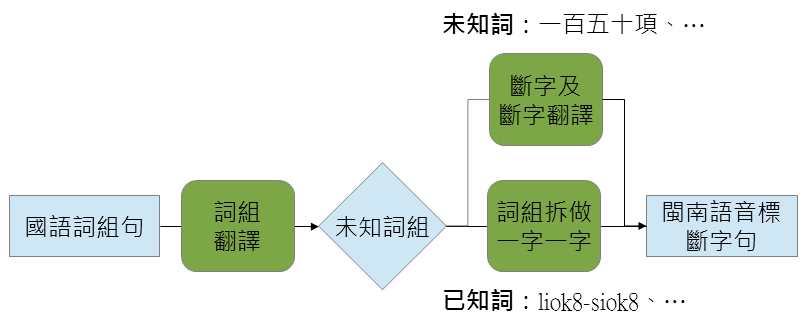
\includegraphics[keepaspectratio,width=40em]{圖/未知詞另外翻譯}}
\caption{未知詞另外翻譯流程}
\label{未知詞另外翻譯}
\end{figure}

對\ref{節:未知詞問題}節來看,
用斷詞翻譯會拄著未知詞的問題。
佇遮阮提出一个演算法\ref{方法:未知詞另外翻譯方法},
準若阮用斷詞翻譯模型,
拄著未知詞的時陣,
這个未知詞會使提予斷字翻譯模型去翻譯。

可比講「陸續 開放 一百五十項 的 規費」提予斷詞組模型翻譯,
得著「liok8-siok8 khai1-hong3 一百五十項 e5 規費」,
閣來共「一百五十項」佮「規費」這兩个詞組切做斷字「一 百 五 十 項」佮「規 費」,
閣擲去斷字模型翻譯,流程會當看圖\ref{未知詞另外翻譯}。

\begin{algorithm}
  \caption{未知詞另外翻譯}
  \label{方法:未知詞另外翻譯方法}
  \begin{algorithmic}
    \REQUIRE \( 原本華語句H = [h_{1}, h_{2},...] \)
    \ENSURE \( 翻譯閩南語句M = [m_{1}, m_{2},...m_{n}] \)
    \STATE \( M = [m_{1}, m_{2},...m_{n}] \gets 斷詞翻譯H的結果 \)
    
	\WHILE{存在$B = [m_{i} , m_{i+1} ,...m_{j}] 攏是未知詞,m_{i−1}, m_{j+1}是已知詞$}
		\STATE \( T \gets B提去斷字翻譯 \)
		\STATE 共M內的B換做T
	\ENDWHILE
  \end{algorithmic}
\end{algorithm}


\section{漢羅全羅對齊}
\label{節:漢羅全羅對齊}
佇\ref{節:臺文典藏}節有講著,
臺文典藏是提供漢羅佮全羅的對照,
因為阮的翻譯需要一个漢字對一个音標的一對一,
所以愛共臺文典藏伊原本一段對齊一段的語料改做一字對一字。
而且愛注意臺文典藏佇2006年完成,
教育部的漢字規範佇2007年才公佈,
所以\ji{⿰因}兩个的用字規範是無完全仝款的。
毋過臺文典藏的語料倩人整理的時陣內部有訂標準,伊的漢字有一半以上攏是會用得的。
本論文用字以教育部的為主,
對齊的做法是共漢羅逐字攏去對看覓全羅,
看漢羅字一字佮全羅一字的對應有佇字典內底無,
揣出上長的對應組合。

%有1個少年人;伊抵tng7 teh 想
%U7 chit8 e5 siau3-lian5 lang5; i tu2-tng7 teh siuN7 phok-su7 lun7-bun5, 

\section{補全漢佮全羅}
\label{節:補全漢佮全羅}
佇\ref{節:整理語料}節有講著,
閩南語語料的完整資訊有全漢、全羅、斷詞三項,
若全部的語料攏有這三種資訊,
翻譯效果會閣較好。

斷詞的部份佇\ref{節:拄好長度斷詞}節有討論矣,
這節的重點是下佇按怎自動整理語料,
予\ji{⿰因}有完整的全漢佮全羅資訊,
也就是替\ji{⿰因}補起哩欠的漢字佮羅馬音標。

因為有的詞可能一字音標、一字是漢字,
親像「彰化」,寫做「tsiong-化」。
本論文提出一个做法,
整理語料的時猶原用斷詞方法,
毋過用的辭典愛小可仔改變,
逐个詞的全部形式攏愛加佇辭典內底,
閣愛加
「\tsoo{彰}{}{}\tsoo{化}{}{}」、
「\tsoo{彰}{}{}\tsoo{huà}{}{}」、
「\tsoo{彰}{}{}\tsoo{化}{⿳⿳⿳ㄏㄨㄚ˪}{huà}」、
「\tsoo{tsiong}{}{}\tsoo{化}{}{}」、
「\tsoo{tsiong}{}{}\tsoo{huà}{}{huà}」、
「\tsoo{tsiong}{}{}\tsoo{化}{}{}」、
「\tsoo{彰}{⿳⿳ㄐㄧㆲ}{tsiong}\tsoo{化}{}{}」、
「\tsoo{彰}{⿳⿳ㄐㄧㆲ}{tsiong}\tsoo{huà}{}{}」、
「\tsoo{彰}{⿳⿳ㄐㄧㆲ}{tsiong}\tsoo{化}{⿳⿳⿳ㄏㄨㄚ˪}{huà}」
%「\tsoo{彰}{}{}\tsoo{化}{}{}」、
%「\tsoo{彰}{}{}\tsoo{}{⿳⿳⿳ㄏㄨㄚ˪}{huà}」、
%「\tsoo{彰}{}{}\tsoo{化}{⿳⿳⿳ㄏㄨㄚ˪}{huà}」、
%「\tsoo{}{⿳⿳ㄐㄧㆲ}{tsiong}\tsoo{化}{}{}」、
%「\tsoo{}{⿳⿳ㄐㄧㆲ}{tsiong}\tsoo{}{⿳⿳⿳ㄏㄨㄚ˪}{huà}」、
%「\tsoo{}{⿳⿳ㄐㄧㆲ}{tsiong}\tsoo{化}{⿳⿳⿳ㄏㄨㄚ˪}{huà}」、
%「\tsoo{彰}{⿳⿳ㄐㄧㆲ}{tsiong}\tsoo{化}{}{}」、
%「\tsoo{彰}{⿳⿳ㄐㄧㆲ}{tsiong}\tsoo{}{⿳⿳⿳ㄏㄨㄚ˪}{huà}」、
%「\tsoo{彰}{⿳⿳ㄐㄧㆲ}{tsiong}\tsoo{化}{⿳⿳⿳ㄏㄨㄚ˪}{huà}」
攏總九種\footnote{一个字的資訊可能是「漢字」、「音標」、「漢字音標攏有」三種其中一種。
兩字,攏總$3^{2}=9$種}。

%為著查字典的速度閣較緊,
%就親像圖XX仝款,
%逐个詞一字一字處理落來,
%逐字分做漢字、音標、一對一三个點,
%第二个字閣佇這三个點閣生落去,
%毋過第一个字有佮別的詞仝款,
%就會使公家一个點,
%親像「彰化」「將來」「將軍庄」,
%因為限制上長四字詞\footnote{照教育部的「臺灣閩南語羅馬字拼音方案連字符使用原則」,
%有可能有五字詞,毋過這擺實驗限制四字詞},
%一个詞上濟產生120點\footnote{第一層加到第四層,$3^{1}+3^{2}+3^{3}+3^{4}=120$},
%毋過揣候選詞的時間複雜度是$O(1)$。

決定斷詞斷佇佗位了後,
逐个斷詞的所在可能有超過一个的候選詞,
%「彰化的米誠好食」,
上尾閣用語言模型,
配合維特比算法,
揀出機率上懸的語句。


\section{語言分類特徵}
\label{節:語言分類特徵}

\ref{節:語言分類}節有講,
閩南語佮華語以字為單位的語言模型效果無好,
為著予電腦會當分別閩南語佮華語,
阮就愛準備幾項閩南語佮華語無仝的特徵。
本論文提出一个以斷詞資訊做判斷特徵的方法,
除了以斷詞算語言模型以外,
閣加入斷詞了一字詞、兩字詞、三字詞、四字詞的詞數,
毋過按呢猶原無夠。

閩南語佮華語上大差別就是用詞無仝,
閩南語寫「食飯」、「無法度」,
華語寫「吃飯」、「沒辦法」,
所以阮揀定用詞出來,
當作阮的特徵之一。

毋過閩南語佮華語有誠濟共同詞,
親像「火車」、「電腦」,
\ji{⿰因}寫法是仝款的,
阮袂使直接提定用詞來做,
因為內底會有共同詞,
所以阮愛揀出無共同詞的「特徵詞」。

選特徵詞的方法是先統計閩南語語料佮華語語料,
分別揣出n个定用詞\footnote{有算標點符號},
了後揀出頭前m个閩南語定用詞,
而且這m个閩南語定用詞無出現佇華語n个定用詞,
這m个詞阮就號做閩南語特徵詞。
華語部份嘛仝款,
揀出頭前m个華語定用詞,
這m个詞無出現佇閩南語的n个定用詞,
這m个詞就是華語的特徵詞。

佇遮阮設$定用詞數量是n=7000,特徵詞數量是m=3000$來揣華語閩南語的特徵詞,
頭幾个定用詞佮特徵詞佇表\ref{表:定用詞佮特徵詞},
「\tsoo{的}{⿳ㆤˊ}{ê}」佮「\tsoo{伊}{⿳ㄧ }{i}」攏是閩南語的定用詞,
毋過這兩个詞「\tsoo{的}{⿳⿳˙ㄉㄜ}{}」佮「\tsoo{伊}{⿳ㄧ }{}」華語攏會用著,
所以袂使做閩南語的特徵詞。
親像「\tsoo{佇}{⿳⿳ㄉㄧ˫}{tī}」華語就罕得用著「\tsoo{佇}{⿳⿳ㄓㄨˋ}{}」,
就會使當做閩南語的特徵詞。

有斷詞、語言模型佮特徵詞的資訊,
就會當親像圖\ref{圖:判斷語言架構}仝款,
交予分類器做語言分類。

\begin{table}
\caption{n=7000、m=3000的頭前九个定用詞佮特徵詞}
\label{表:定用詞佮特徵詞}
\centering
\begin{tabular}{c|cccccccccc}
第幾个 & 1 & 2 & 3 & 4 & 5 & 6 & 7 & 8 & 9\\
\hline
閩南語定用詞 &
\tsoo{的}{⿳ㆤˊ}{ê} & \tsoo{伊}{⿳ㄧ }{i} & \tsoo{有}{⿳ㄨ˫}{ū} &
\tsoo{是}{⿳⿳ㄒㄧ˫}{sī} & \tsoo{我}{⿳⿳⿳ㆣㄨㄚˋ}{guá} & \tsoo{人}{⿳⿳ㄌㄤˊ}{lâng} &
\tsoo{無}{⿳⿳ㆠㄜˊ}{bô} & \tsoo{講}{⿳⿳ㄍㆲˋ}{kóng} & \tsoo{佇}{⿳⿳ㄉㄧ˫}{tī} & …\\
\hline
華語定用詞 &
\tsoo{的}{⿳⿳˙ㄉㄜ}{} & \tsoo{是}{⿳ㄕˋ}{} & \tsoo{在}{⿳⿳ㄗㄞˋ}{} &
\tsoo{一}{⿳ㄧ }{} & \tsoo{有}{⿳⿳ㄧㄡˇ}{} & \tsoo{了}{⿳⿳˙ㄌㄜ}{} &
\tsoo{不}{⿳⿳ㄅㄨˋ}{} & \tsoo{我}{⿳⿳ㄨㄛˇ}{} & \tsoo{個}{⿳⿳˙ㄍㄜ}{} & …\\
\hline
閩南語特徵詞 &
\tsoo{佇}{⿳⿳ㄉㄧ˫}{tī} & \tsoo{个}{⿳ㆤˊ}{ê} & \tsoo{閣}{⿳⿳ㄍㄜㆷ}{koh} &
\tsoo{攏}{⿳⿳ㄌㆲˋ}{lóng} & \tsoo{佮}{⿳⿳ㄍㄚㆴ}{kap} & \tsoo{\ji{⿰因}}{⿳ㄧㄣ}{in} &
\tsoo{咧}{⿳⿳ㄉㆤㆷ}{teh} & \tsoo{咱}{⿳⿳ㄌㄢˋ}{lán} & \tsoo{彼}{⿳⿳ㄏㄧㆵ}{hit} & …\\
\hline
華語特徵詞 &
\tsoo{我}{⿳⿳ㄨㄛˇ}{}\tsoo{們}{⿳⿳˙ㄇㄣ}{} & \tsoo{很}{⿳⿳ㄏㄣˇ}{} & \tsoo{她}{⿳ㄊㄚ}{} &
\tsoo{沒}{⿳⿳ㄇㄟˊ}{}\tsoo{有}{⿳⿳ㄧㄡˇ}{} & \tsoo{或}{⿳⿳⿳ㄏㄨㄛˋ}{} & \tsoo{他}{⿳ㄊㄚ}{}\tsoo{們}{⿳⿳˙ㄇㄣ}{} &
\tsoo{更}{⿳⿳ㄍㄥˋ}{} & \tsoo{則}{⿳⿳ㄗㄜˊ}{} & \tsoo{把}{⿳⿳ㄅㄚˇ}{} & …\\
\end{tabular}
\end{table}

\begin{figure}
\centerline{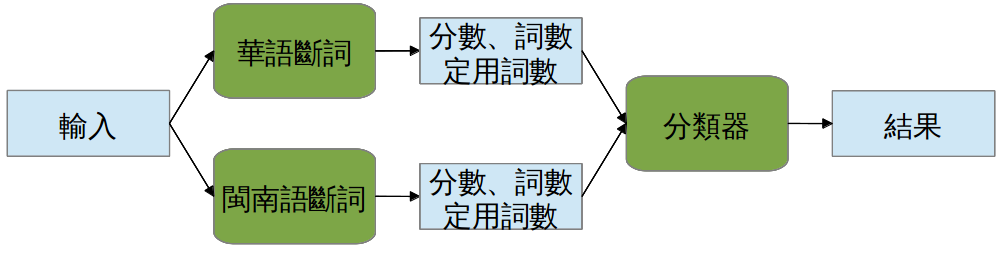
\includegraphics[keepaspectratio,width=40em]{圖/判斷語言架構}}
\caption{判斷語言流程}
\label{圖:判斷語言架構}
\end{figure}


\chapter{實驗結果}
\label{章:實驗結果}
SRILM 1.7.0
GIZA++ 1.0.7
Moses 40c819d285cdeb40c0b8cc428bfde2fcb531b655
臺灣言語工具 0.5.0
為著逐家後壁研究的方便,本論文研究的過程佮結果,全部公開佇網路頂\footnote{\url{https://github.com/sih4sing5hong5/huan1-ik8_gian5-kiu3.git}},詳細按怎用請看附錄\ref{章:按怎裝程式}。

\section{閩南語斷詞實驗}
\label{節:閩南語斷詞實驗}

\begin{table}
\caption{閩南語斷詞的效果}
\label{表:閩南語斷詞的效果}
\centering
\begin{tabular}{c|ccc}
斷詞方法 & 召回率 & 精確率 & F測量\\
\hline
拄好長度斷詞 & 91.1 & 85.1 & 88.0\\
長詞優先斷詞(對頭前) & 91.0 & 84.9 & 87.9\\
長詞優先斷詞(對後壁) & 91.1 & 85.0 & 88.0\\
\end{tabular}
\end{table}

本實驗是提教育部辭典的35130个詞條當做訓練語料,
試驗語料是教育部辭典例句8027句。
共試驗語料的斷詞資訊提掉了後,
用拄好長度斷詞佮長詞優先去斷詞,
才閣佮原本例句的斷詞比較,
得著表\ref{表:閩南語斷詞的效果}的結果。

會當看著拄好長度斷詞的分數有比長詞優先閣較好淡薄,
毋過無明顯的進步。
這兩種斷詞方法的精確率攏比召回率低誠濟,
代表辭典內底收的詞閣無夠濟。

\section{語料整理實驗}
\label{節:語料整理實驗}

\begin{table}
\caption{新聞語料庫佮數位典藏互相整理的實驗}
\label{表:互相整理實驗}
\centering
\begin{tabular}{lcccccc}
整理幾擺 & 原始語料 & 1 & 2 & 3 & 4 & 5\\
BLEU分數 & 9.30 & 14.72 & 13.77 & 13.82 & 13.82 & 13.82\\
\end{tabular}
\end{table}

完整的閩南語語料愛有全漢、全羅佮斷詞資訊。
因為新聞語料庫有全漢、全羅,無斷詞,數位典藏有斷詞毋過無完整的全漢佮全羅。
%,教育部辭典斷詞佮全漢全羅攏有。
%攏就會使用教育部辭典佮數位典藏共新聞語料庫斷詞,閣共斷好的新聞語料庫佮教育部辭典提來標數位典藏的一對一,閣重做幾仔擺,到收斂為止,親像圖XX。

本實驗是提教育部辭典的35130个詞條佮附錄388句當做標準語料,
用拄好長度斷詞來整理新聞平行語料64121句佮數位典藏329476句。
而且用詞為單位拍分數。

表\ref{表:互相整理實驗}是整理的結果,
整理的結果一息仔就收斂,
會當看著整理了的分數比猶未整理前好欲一半。
毋過整理第二擺了後,分數有降一寡,
看整理了的結果,
是因為新聞佮典藏內底的攏有一寡錯誤,
所以第二擺用著遮的資料,
會影響著整理的結果。

%人-為|jin5-ui5 的|e5
%人-為-的|jin5-ui5-e5


\section{分類語言實驗}
\label{節:判斷語言實驗}

\begin{figure}
\caption{無仝特徵詞數量,分類3741段閩南語華語}
\label{圖:無仝特徵詞數量對分類閩南語華語效果的影響}
\begin{tikzpicture}
\begin{axis}[
scaled y ticks=real:1,
ytick scale label code/.code={},
ymax = 14,
symbolic x coords={0,10,20,50,100,200,500,1000,2000,3000},
xtick=data,
height=8cm,
width=14cm,
grid=major,
xlabel={特徵詞數量},
ylabel={分類錯誤率},
legend style={
cells={anchor=east},
legend pos=north east,
%mark size=0.5em
}
]
\addplot coordinates {
(0,13.79) (10,6.87) (20,5.45) (50,4.12)
(100,3.88) (200,3.90) (500,4.12)
(1000,3.80) (2000,4.14) (3000,4.14)
%(0,516) (10,257) (20,204) (50,154)
%(100,145) (200,146) (500,154)
%(1000,142) (2000,155) (3000,155)
};

\legend{SVM}
\end{axis}
\end{tikzpicture}
\end{figure}

這節實驗的語料是對TGB通訊創刊開始,到2014年6月12日為止攏總177期1179篇文章,
提出頭前1000篇做訓練語料,閩南語有9368段488844詞,華語有8519段439436詞;
後壁179篇做訓練語料,閩南語有1344段75282詞,華語有2397段114901詞。
以段做辨識單位,提來予支援向量機分類。

毋過6012个特徵實在是傷濟矣,所以咱試看覓共3000特徵詞減少,看會影響著辨識率無。
實驗結果佇表\ref{圖:無仝特徵詞數量對分類閩南語華語效果的影響},
佇50~100个特徵詞分類效果就收斂矣,加閣較濟的特徵詞,無啥影響著辨識的效果。

\section{加入TGB語料庫實驗}
\label{節:加入TGB語料庫實驗}

\begin{table}
\caption{加入TGB語料的翻譯效果}
\label{表:加入TGB語料的翻譯效果}
\centering
\begin{tabular}{lcccccc}
& 加TGB語料前 & 加TGB語料後\\
平行語料句數 & 64121句 & 99146句\\
BLEU分數 & 13.82 & 19.33\\
\end{tabular}
\end{table}

頂一節做分類語言的實驗,
紲落來就是共TGB語料摻入來翻譯語料。

先提教育部詞條佮附錄句和
\ref{節:語料整理實驗}節整理了的新聞佮典藏語料
來整理TGB語料,
閣用Bleualign來對齊,
就會使提著35025句TGB平行語料。

實驗訓練語料除了\ref{節:語料整理實驗}節的語料外,
閣加入TGB平行語料,
除了教育部附錄句、典藏干焦會使做語言模型以外,
原本平行語料干焦是新聞語料庫64121句,
加入TGB語料35025句了後變做99146句,
對表\ref{表:加入TGB語料的翻譯效果}會當看著進步誠濟,
代表平行語料閣無夠,
閣佇加語料就會使幫助翻譯的階段。
%母語愛專注佇語料處理

\section{斷詞樣式佮斷字樣式的翻譯結果實驗}
\label{節:斷詞樣式佮斷字樣式的翻譯結果實驗}


\begin{figure}
\caption{斷字佮斷詞語料的翻譯效果比較}
\label{圖:斷字佮斷詞語料的翻譯效果比較}
\begin{tikzpicture}
    \begin{axis}[
        width  = 0.85*\textwidth,
        height = 8cm,
        major x tick style = transparent,
        x tick label style={rotate=30,anchor=east},
        ybar=2*\pgflinewidth,
        bar width=14pt,
        ymajorgrids = true,
        ylabel = {BLEU分數},
        symbolic x coords={華語斷字-閩南語斷字,華語斷字-閩南語斷詞,華語斷詞-閩南語斷字,華語斷詞-閩南語斷詞},
        xtick = data,
        enlarge x limits=0.25,
%        scaled y ticks = false,
       % ymin=0,
%        legend cell align=left,
%        legend style={
%                at={(1,1.05)},
%                anchor=south east,
%                column sep=1ex
%        }
    ]
        \addplot
            coordinates {(華語斷字-閩南語斷字, 31.85) (華語斷字-閩南語斷詞,31.24)
  	          (華語斷詞-閩南語斷字,30.74) (華語斷詞-閩南語斷詞,29.22)};
        \addplot
            coordinates {(華語斷字-閩南語斷字, 31.85) (華語斷字-閩南語斷詞,31.26)
  	          (華語斷詞-閩南語斷字,31.90) (華語斷詞-閩南語斷詞,30.92)};
        \addplot
            coordinates {(華語斷字-閩南語斷字, 31.85) (華語斷字-閩南語斷詞,31.24)
  	          (華語斷詞-閩南語斷字,31.44) (華語斷詞-閩南語斷詞,30.43)};
        \legend{無處理未知詞,斷字-斷字翻譯,斷字-斷詞翻譯}
    \end{axis}
\end{tikzpicture}
\end{figure}

為著愛比較華語佮閩南語

這个實驗的訓練、試驗語料佮頂一个實驗是仝款的,
只是上尾是用字做單位來算BLEU分數,
所以圖\ref{圖:斷字佮斷詞語料的翻譯效果比較}的實驗分數看起來會較懸,
並毋是翻譯的效果較好。

這个實驗會當看著兩件代誌,
第一件是未知詞若有處理,
對翻譯有幫助,
而且未知詞用「華語斷字-閩南語斷字」的效果比「華語斷字-閩南語斷詞」閣較好,
可能是因為未知詞大部份攏是需要一字一字照翻的,
嘛有可能是語料無夠濟,
斷字對斷字的統計數量較濟。

第二件代誌是華語的斷詞對翻譯有幫助,
毋過閩南語的斷詞煞無。
可能是閩南語的斷詞閣無夠準,
造成翻譯效果變\ji{⿰禾黑}。

這个實驗是用字做比較單位,
雖然華語斷詞配閩南語斷字的成績上好,
若佇需要斷詞的環境下\footnote{親像語音合成},
閣愛算落斷詞效果可能無好,
效果會拍折。
\chapter{結論佮未來發展}
\label{章:結論佮未來發展}
目前臺灣的本土語言佇沓沓仔流失,
需要逐家用心來注意,
這嘛是這篇論文研究華語翻譯到閩南語的上主要目的。
下跤會盡量共經驗分享予其他母語,
希望閩南語以外,
客話佮咱的原住民南島語,
嘛會使利用這个研究成果。

\section{結論}
\label{節:結論}
本論文提出「拄好長度斷詞」的方法,
試圖改善「長詞優先」的缺點,
毋過佇\ref{節:閩南語斷詞實驗}節的實驗內底,
對無濟訓練語料來講,
兩種斷詞方法的效果略略仔爾。

%斷詞的影響
%客話

佇\ref{節:語料整理實驗}節佮\ref{節:加入TGB語料庫實驗}節的實驗,
會當看著整理閩南語的效果,
對原本的9.30分加到19.33分,
代表對閩南語來講,
這馬無夠十萬句的語料,
是翻譯效果\ji{⿰禾黑}的一大限制。
對臺灣別的本土語言來講,
語料數量是一个上大的問題。

分類華語佮閩南語兩種語言佇\ref{節:判斷語言實驗}節嘛有$96\%$正確的成績,
若愛一擺分類三種以上n个漢語,
會使簡化做兩種漢語的分類,
先共n个語言,
兩个兩个語言彼此之間揣出特徵詞,
訓練出$\frac{n\times(n-1)}{2}$个分類模型,
上尾投票,
看佗一个語言贏較濟,
就當作是彼个語言。

可比講這馬有閩南語、客家四縣話、客家饒平話、佮華語四種語言愛分類,
先訓練「閩南語-客家四縣話」、「閩南語-客家饒平話」、「閩南語-華語」、
「客家四縣話-客家饒平話」、「客家四縣話-華語」、「客家饒平話-華語」六个模型,
閣來共試驗語料提入來予六个模型判斷,
分別判斷出「客家四縣話」、「客家饒平話」、「閩南語」、
「客家饒平話」、「客家四縣話」、「客家饒平話」,
看這六个模型分類內底「客家饒平話」上濟,
就判斷做「客家饒平話」的語料。
準做有需要分類南島語,會當看\ref{小節:語言分類}節的說明。

紲落來講兩个會當加強翻譯的方法,佮一个翻譯模型會當閣利用的所在:
\section{鬥相共人工校對}
\label{節:鬥相共人工校對}

%圖:鬥相共人工校對
\ref{節:語料整理實驗}節的實驗結果共咱講,
就算咱提著的語料毋是蓋完整,
咱嘛會當補足伊的資訊,
予翻譯變好。
這嘛表示語料正確度對翻譯有影響,
用機器整理語料有伊的限制,
若愛予語料正確,
一定就需要人工校對。

%抑是用有一對一較完整的資料去鬥處理,攏會使予翻譯的效果閣較好。
%毋過完整的資料數量若較濟,翻譯的效果會愈好。

%準做資料是親像數位典藏仝款補一部份漢字爾仔,嘛是愛人工閣巡一擺,其他漢羅抑是全羅的用電腦自動標一對一了後,閣較需要人工共⿰因閣校對過。
%愛有完整一對一資料,人工是走袂去的,親像圖X仝款,咱有完整的資料,去標猶未整理的語料,經過人工檢查了後,完整的資料就閣較濟,按呢標一對一就閣較準,就無需要遮爾濟的人工,創造一个好的循環。

毋過人工校對是開錢開時間開氣力的代誌,
人工校對上驚無彩工一直改仝款的語料錯誤,
機器整理模型就愛綴咧改,
予錯誤較少,
毋過嘛有可能予原本整理著的語料變做錯誤,
所以會當閣準備一个鬥相共的工具,
予整理模型改變時,
原本整理著的語料袂變毋著,
才有法度。

%親像圖XX
準做有改錯字工具,
予標一對一的正確率閣較懸,
就會減少人工檢查的負擔。
人工檢查前的輸入佮人工檢查了的輸出,
嘛會使做一个改錯字的系統,
予人免一直改仝款的錯誤。

毋管是標全漢全羅,
抑是斷詞、剖析佮語音資料,
發展技術佮照顧語料對發展閩南語研究來講平平仔重要,
絕對袂使重視技術煞袂記得語料。

%\subsection{重斷數位典藏}
%\label{節:重斷數位典藏}
%數位典藏有的斷詞其實毋好,親像「」應該是兩个詞

\section{斷詞}
\label{節:未來斷詞}
%看楊允言
華語斷詞是一个發展足完整的技術\footnote{CKIP正確率%},毋過閩南語的語料毋華語遐爾濟的人工,就會影響著效果。
本論文是用對「上長度優先」的算法改做「拄好長度斷詞」\footnote{請看\ref{節:拄好長度斷詞}節},嘛會使閣用統計方法看斷詞的效果會較好無。
用統計的方法會使用翻譯工具來做,一字一字斷字的輸入配合一詞一詞斷詞的輸出,提去訓練翻譯模型,按呢就有一个統計的斷詞工具。
到底佗一个方法佇閩南語、客話這種幾萬、幾十萬句語料,效果會閣較好,就需要閣一寡研究矣。
\section{剖析}
\label{節:未來剖析}
%看楊允言
楊允言教授捌做過閩南語的剖析,毋過需要語言學的知識,閣有一致的人工檢查,而且一開始的語料歹收集,可能著的先共閩南語翻譯做華語,才閣共華語語句的剖析結果\footnote{中研院剖析}對應轉去閩南語語句,按呢就有初步的資料矣。
訂好規則了後,就需要訂好剖析的規則
人工若校對,全部的資料著愛收集起來
而且嘛愛親像XX節的XX圖仝款,愛做一个改錯誤的程式,予人工莫一直改仝款的物件
等待資料有夠濟,就會提樹仔的語料來訓練一个閩南語的剖析器\footnote{star ford parser}


\section{語音辨識}
\label{節:未來辨識}
字幕 華語字→閩南語字

\bibliographystyle{IEEEtran}
\bibliography{參考文獻}

%\begin{appendices}
%
%\chapter{臺灣言語工具}
\label{章:臺灣言語工具}
臺灣言語工具\cite{臺灣言語工具}
%
%\end{appendices}

\end{document}
